% Options for packages loaded elsewhere
\PassOptionsToPackage{unicode}{hyperref}
\PassOptionsToPackage{hyphens}{url}
\PassOptionsToPackage{dvipsnames,svgnames,x11names}{xcolor}
%
\documentclass[
  10pt,
  letterpaper,
  DIV=11,
  numbers=noendperiod]{scrartcl}

\usepackage{amsmath,amssymb}
\usepackage{iftex}
\ifPDFTeX
  \usepackage[T1]{fontenc}
  \usepackage[utf8]{inputenc}
  \usepackage{textcomp} % provide euro and other symbols
\else % if luatex or xetex
  \usepackage{unicode-math}
  \defaultfontfeatures{Scale=MatchLowercase}
  \defaultfontfeatures[\rmfamily]{Ligatures=TeX,Scale=1}
\fi
\usepackage{lmodern}
\ifPDFTeX\else  
    % xetex/luatex font selection
  \setmainfont[]{Avenir}
  \setsansfont[]{Avenir}
\fi
% Use upquote if available, for straight quotes in verbatim environments
\IfFileExists{upquote.sty}{\usepackage{upquote}}{}
\IfFileExists{microtype.sty}{% use microtype if available
  \usepackage[]{microtype}
  \UseMicrotypeSet[protrusion]{basicmath} % disable protrusion for tt fonts
}{}
\makeatletter
\@ifundefined{KOMAClassName}{% if non-KOMA class
  \IfFileExists{parskip.sty}{%
    \usepackage{parskip}
  }{% else
    \setlength{\parindent}{0pt}
    \setlength{\parskip}{6pt plus 2pt minus 1pt}}
}{% if KOMA class
  \KOMAoptions{parskip=half}}
\makeatother
\usepackage{xcolor}
\usepackage[margin=1in,heightrounded]{geometry}
\setlength{\emergencystretch}{3em} % prevent overfull lines
\setcounter{secnumdepth}{-\maxdimen} % remove section numbering
% Make \paragraph and \subparagraph free-standing
\ifx\paragraph\undefined\else
  \let\oldparagraph\paragraph
  \renewcommand{\paragraph}[1]{\oldparagraph{#1}\mbox{}}
\fi
\ifx\subparagraph\undefined\else
  \let\oldsubparagraph\subparagraph
  \renewcommand{\subparagraph}[1]{\oldsubparagraph{#1}\mbox{}}
\fi


\providecommand{\tightlist}{%
  \setlength{\itemsep}{0pt}\setlength{\parskip}{0pt}}\usepackage{longtable,booktabs,array}
\usepackage{calc} % for calculating minipage widths
% Correct order of tables after \paragraph or \subparagraph
\usepackage{etoolbox}
\makeatletter
\patchcmd\longtable{\par}{\if@noskipsec\mbox{}\fi\par}{}{}
\makeatother
% Allow footnotes in longtable head/foot
\IfFileExists{footnotehyper.sty}{\usepackage{footnotehyper}}{\usepackage{footnote}}
\makesavenoteenv{longtable}
\usepackage{graphicx}
\makeatletter
\def\maxwidth{\ifdim\Gin@nat@width>\linewidth\linewidth\else\Gin@nat@width\fi}
\def\maxheight{\ifdim\Gin@nat@height>\textheight\textheight\else\Gin@nat@height\fi}
\makeatother
% Scale images if necessary, so that they will not overflow the page
% margins by default, and it is still possible to overwrite the defaults
% using explicit options in \includegraphics[width, height, ...]{}
\setkeys{Gin}{width=\maxwidth,height=\maxheight,keepaspectratio}
% Set default figure placement to htbp
\makeatletter
\def\fps@figure{htbp}
\makeatother

\usepackage{booktabs}
\usepackage{longtable}
\usepackage{array}
\usepackage{multirow}
\usepackage{wrapfig}
\usepackage{float}
\usepackage{colortbl}
\usepackage{pdflscape}
\usepackage{tabu}
\usepackage{threeparttable}
\usepackage{threeparttablex}
\usepackage[normalem]{ulem}
\usepackage{makecell}
\usepackage{xcolor}
\usepackage{xcolor}
\definecolor{gis}{HTML}{E69F00}
\definecolor{health}{HTML}{56B4E9}
\definecolor{innovation}{HTML}{CC79A7}
\definecolor{labor}{HTML}{B8860B}
\definecolor{operations}{HTML}{0072B2}
\definecolor{policy}{HTML}{D55E00}
\definecolor{sustainability}{HTML}{009E73}
\definecolor{event}{HTML}{17A2B8}
\usepackage{scrlayer-scrpage}
\pagestyle{scrheadings}
\clearpairofpagestyles
\lohead{\small\textit{\leftmark}}
\KOMAoptions{headsepline=true, footsepline=true}
\KOMAoption{captions}{tableheading}
\makeatletter
\@ifpackageloaded{caption}{}{\usepackage{caption}}
\AtBeginDocument{%
\ifdefined\contentsname
  \renewcommand*\contentsname{Table of contents}
\else
  \newcommand\contentsname{Table of contents}
\fi
\ifdefined\listfigurename
  \renewcommand*\listfigurename{List of Figures}
\else
  \newcommand\listfigurename{List of Figures}
\fi
\ifdefined\listtablename
  \renewcommand*\listtablename{List of Tables}
\else
  \newcommand\listtablename{List of Tables}
\fi
\ifdefined\figurename
  \renewcommand*\figurename{Figure}
\else
  \newcommand\figurename{Figure}
\fi
\ifdefined\tablename
  \renewcommand*\tablename{Table}
\else
  \newcommand\tablename{Table}
\fi
}
\@ifpackageloaded{float}{}{\usepackage{float}}
\floatstyle{ruled}
\@ifundefined{c@chapter}{\newfloat{codelisting}{h}{lop}}{\newfloat{codelisting}{h}{lop}[chapter]}
\floatname{codelisting}{Listing}
\newcommand*\listoflistings{\listof{codelisting}{List of Listings}}
\makeatother
\makeatletter
\makeatother
\makeatletter
\@ifpackageloaded{caption}{}{\usepackage{caption}}
\@ifpackageloaded{subcaption}{}{\usepackage{subcaption}}
\makeatother
\ifLuaTeX
  \usepackage{selnolig}  % disable illegal ligatures
\fi
\usepackage{bookmark}

\IfFileExists{xurl.sty}{\usepackage{xurl}}{} % add URL line breaks if available
\urlstyle{same} % disable monospaced font for URLs
\hypersetup{
  colorlinks=true,
  linkcolor={blue},
  filecolor={Maroon},
  citecolor={Blue},
  urlcolor={Blue},
  pdfcreator={LaTeX via pandoc}}

\author{}
\date{}

\begin{document}

\thispagestyle{empty}
\begin{center}
  
\includegraphics[height=1.4in]{images/logo.png}
\end{center}
\vspace{0.6em}
\begin{center}
{\Huge\textbf{2026 Industry Studies Association}}\\[0.5em]
{\Huge\textbf{Annual Conference}}\\[1em]
{\Large\textit{Program Schedule}}\\[0.4em]
{\large June 3--5, 2026}\\[0.5em]
{\large George Washington University, Washington, DC}
\end{center}
\vspace{1em}
\noindent
\begin{minipage}[t]{0.48\textwidth}
  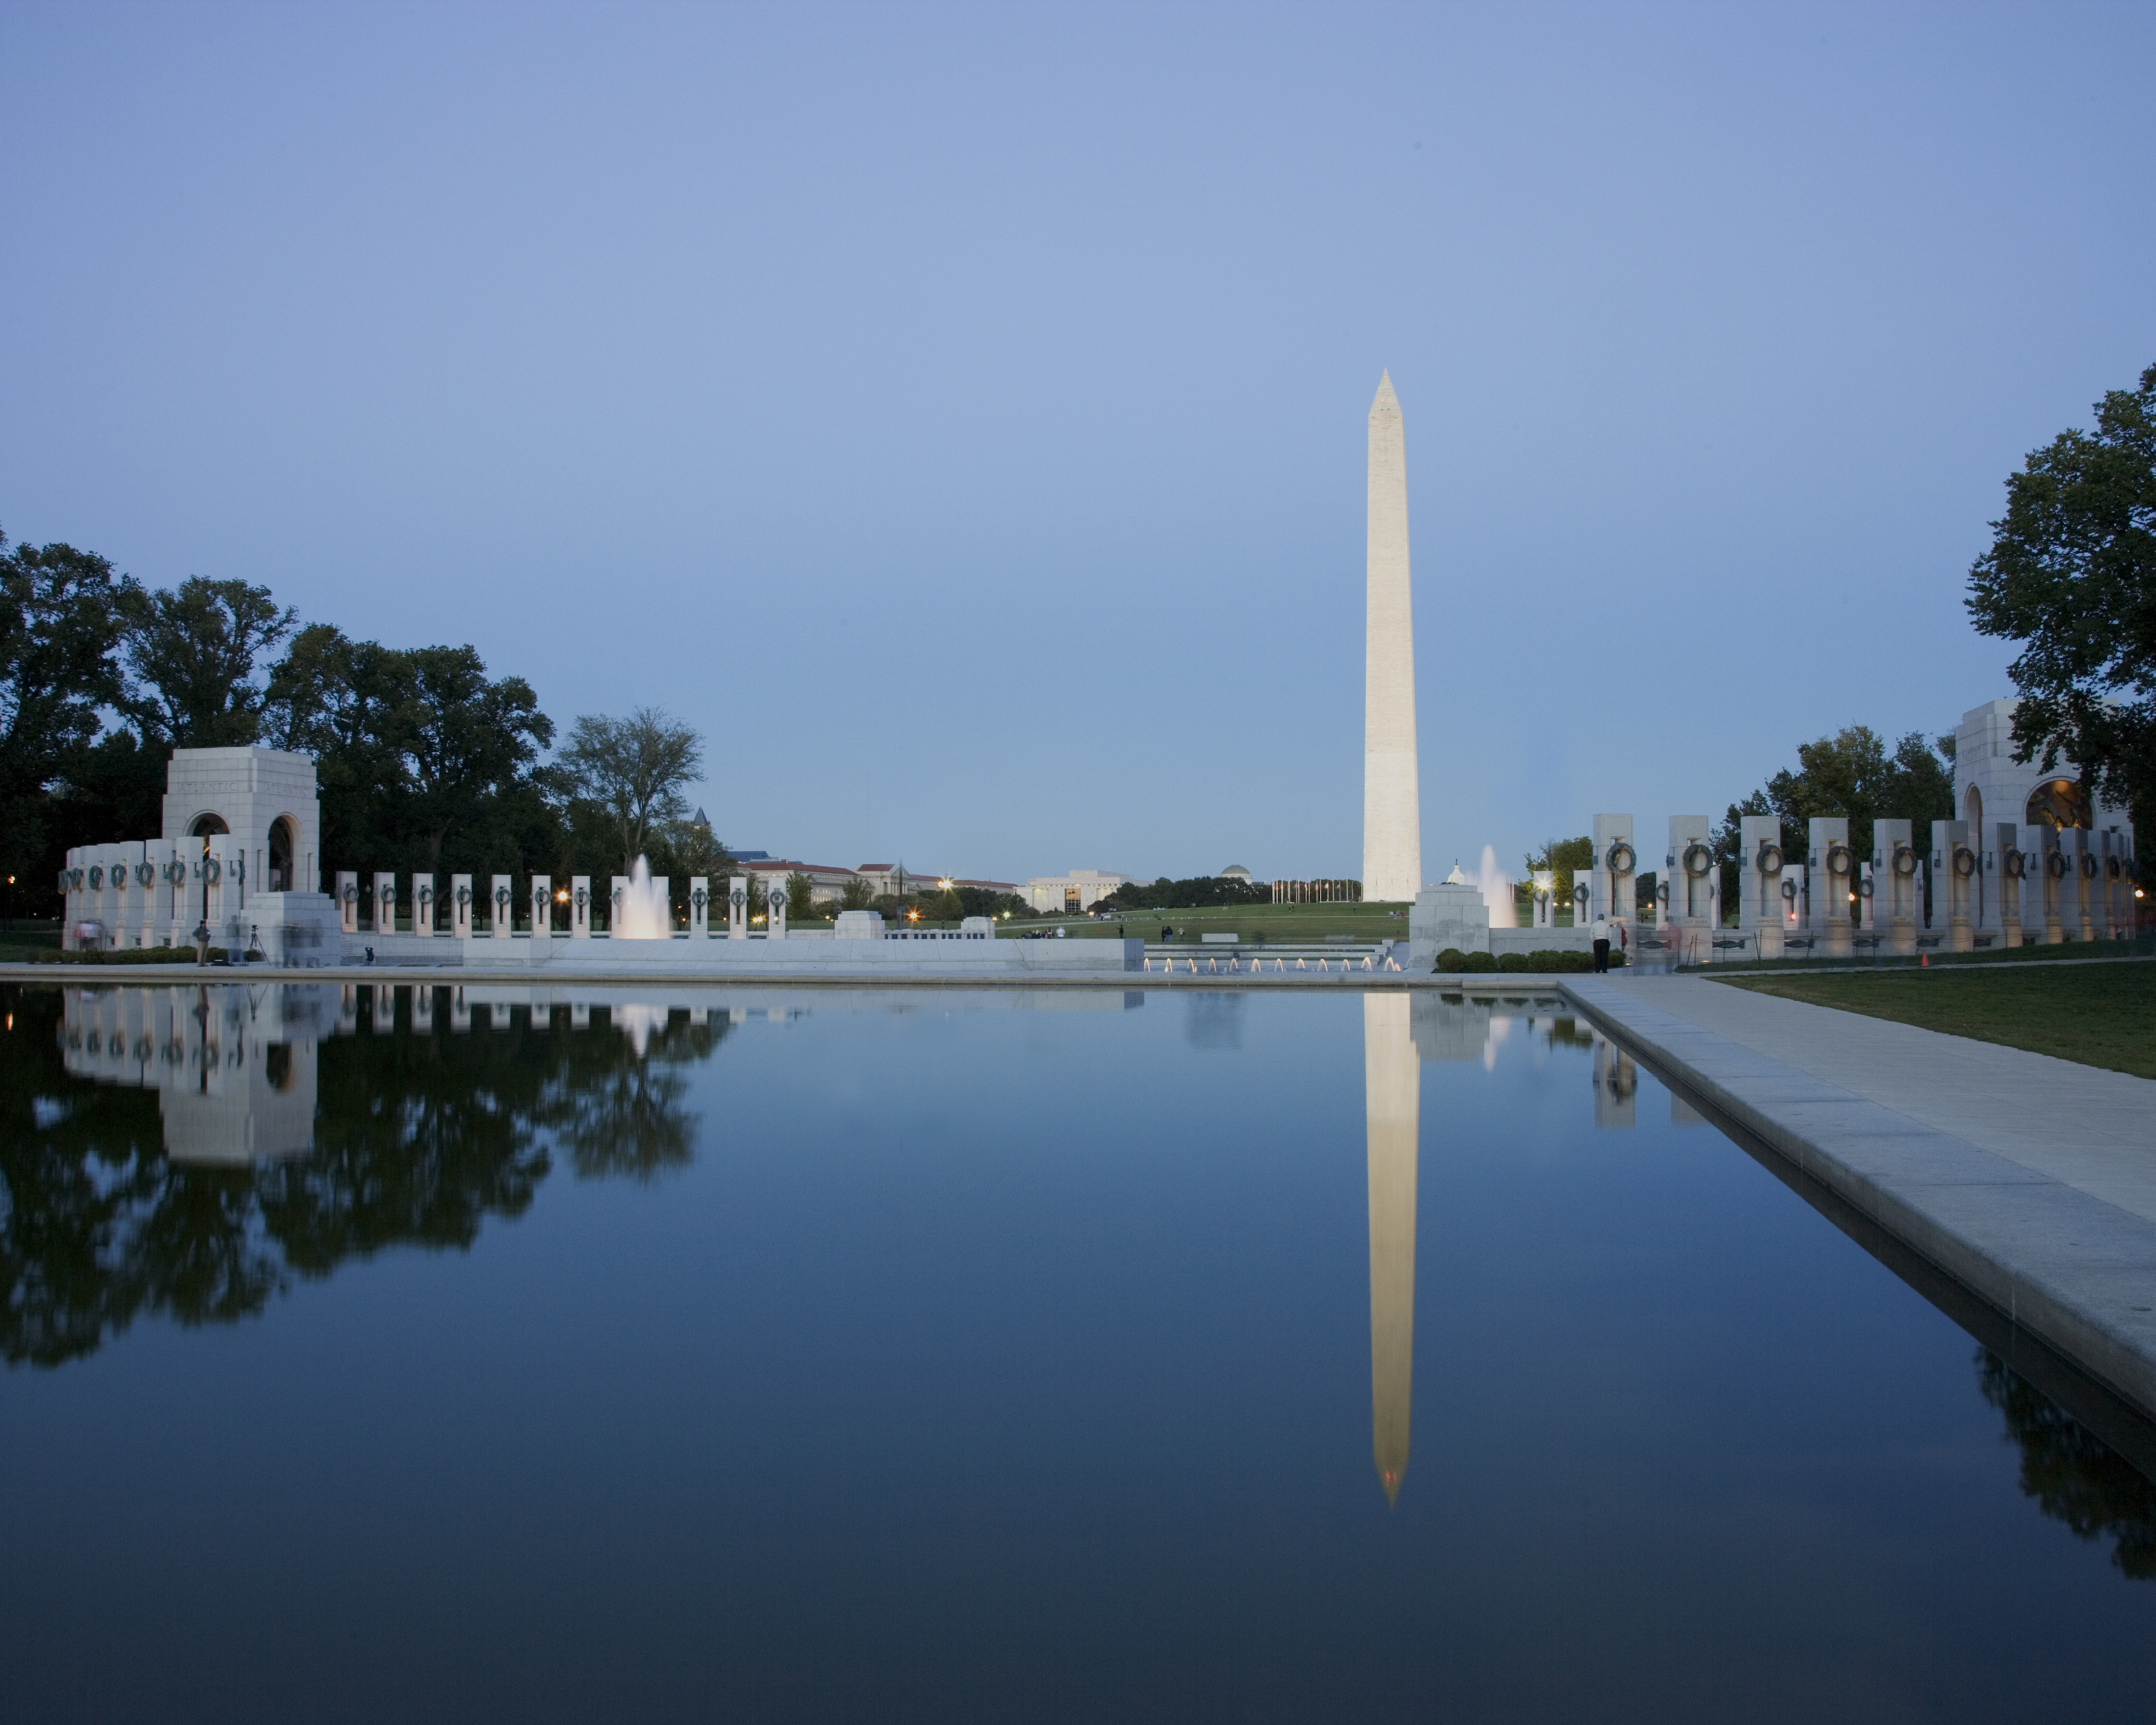
\includegraphics[width=\linewidth]{images/dc/dc_reflecting_pool.jpg}
\end{minipage}\hfill
\begin{minipage}[t]{0.48\textwidth}
  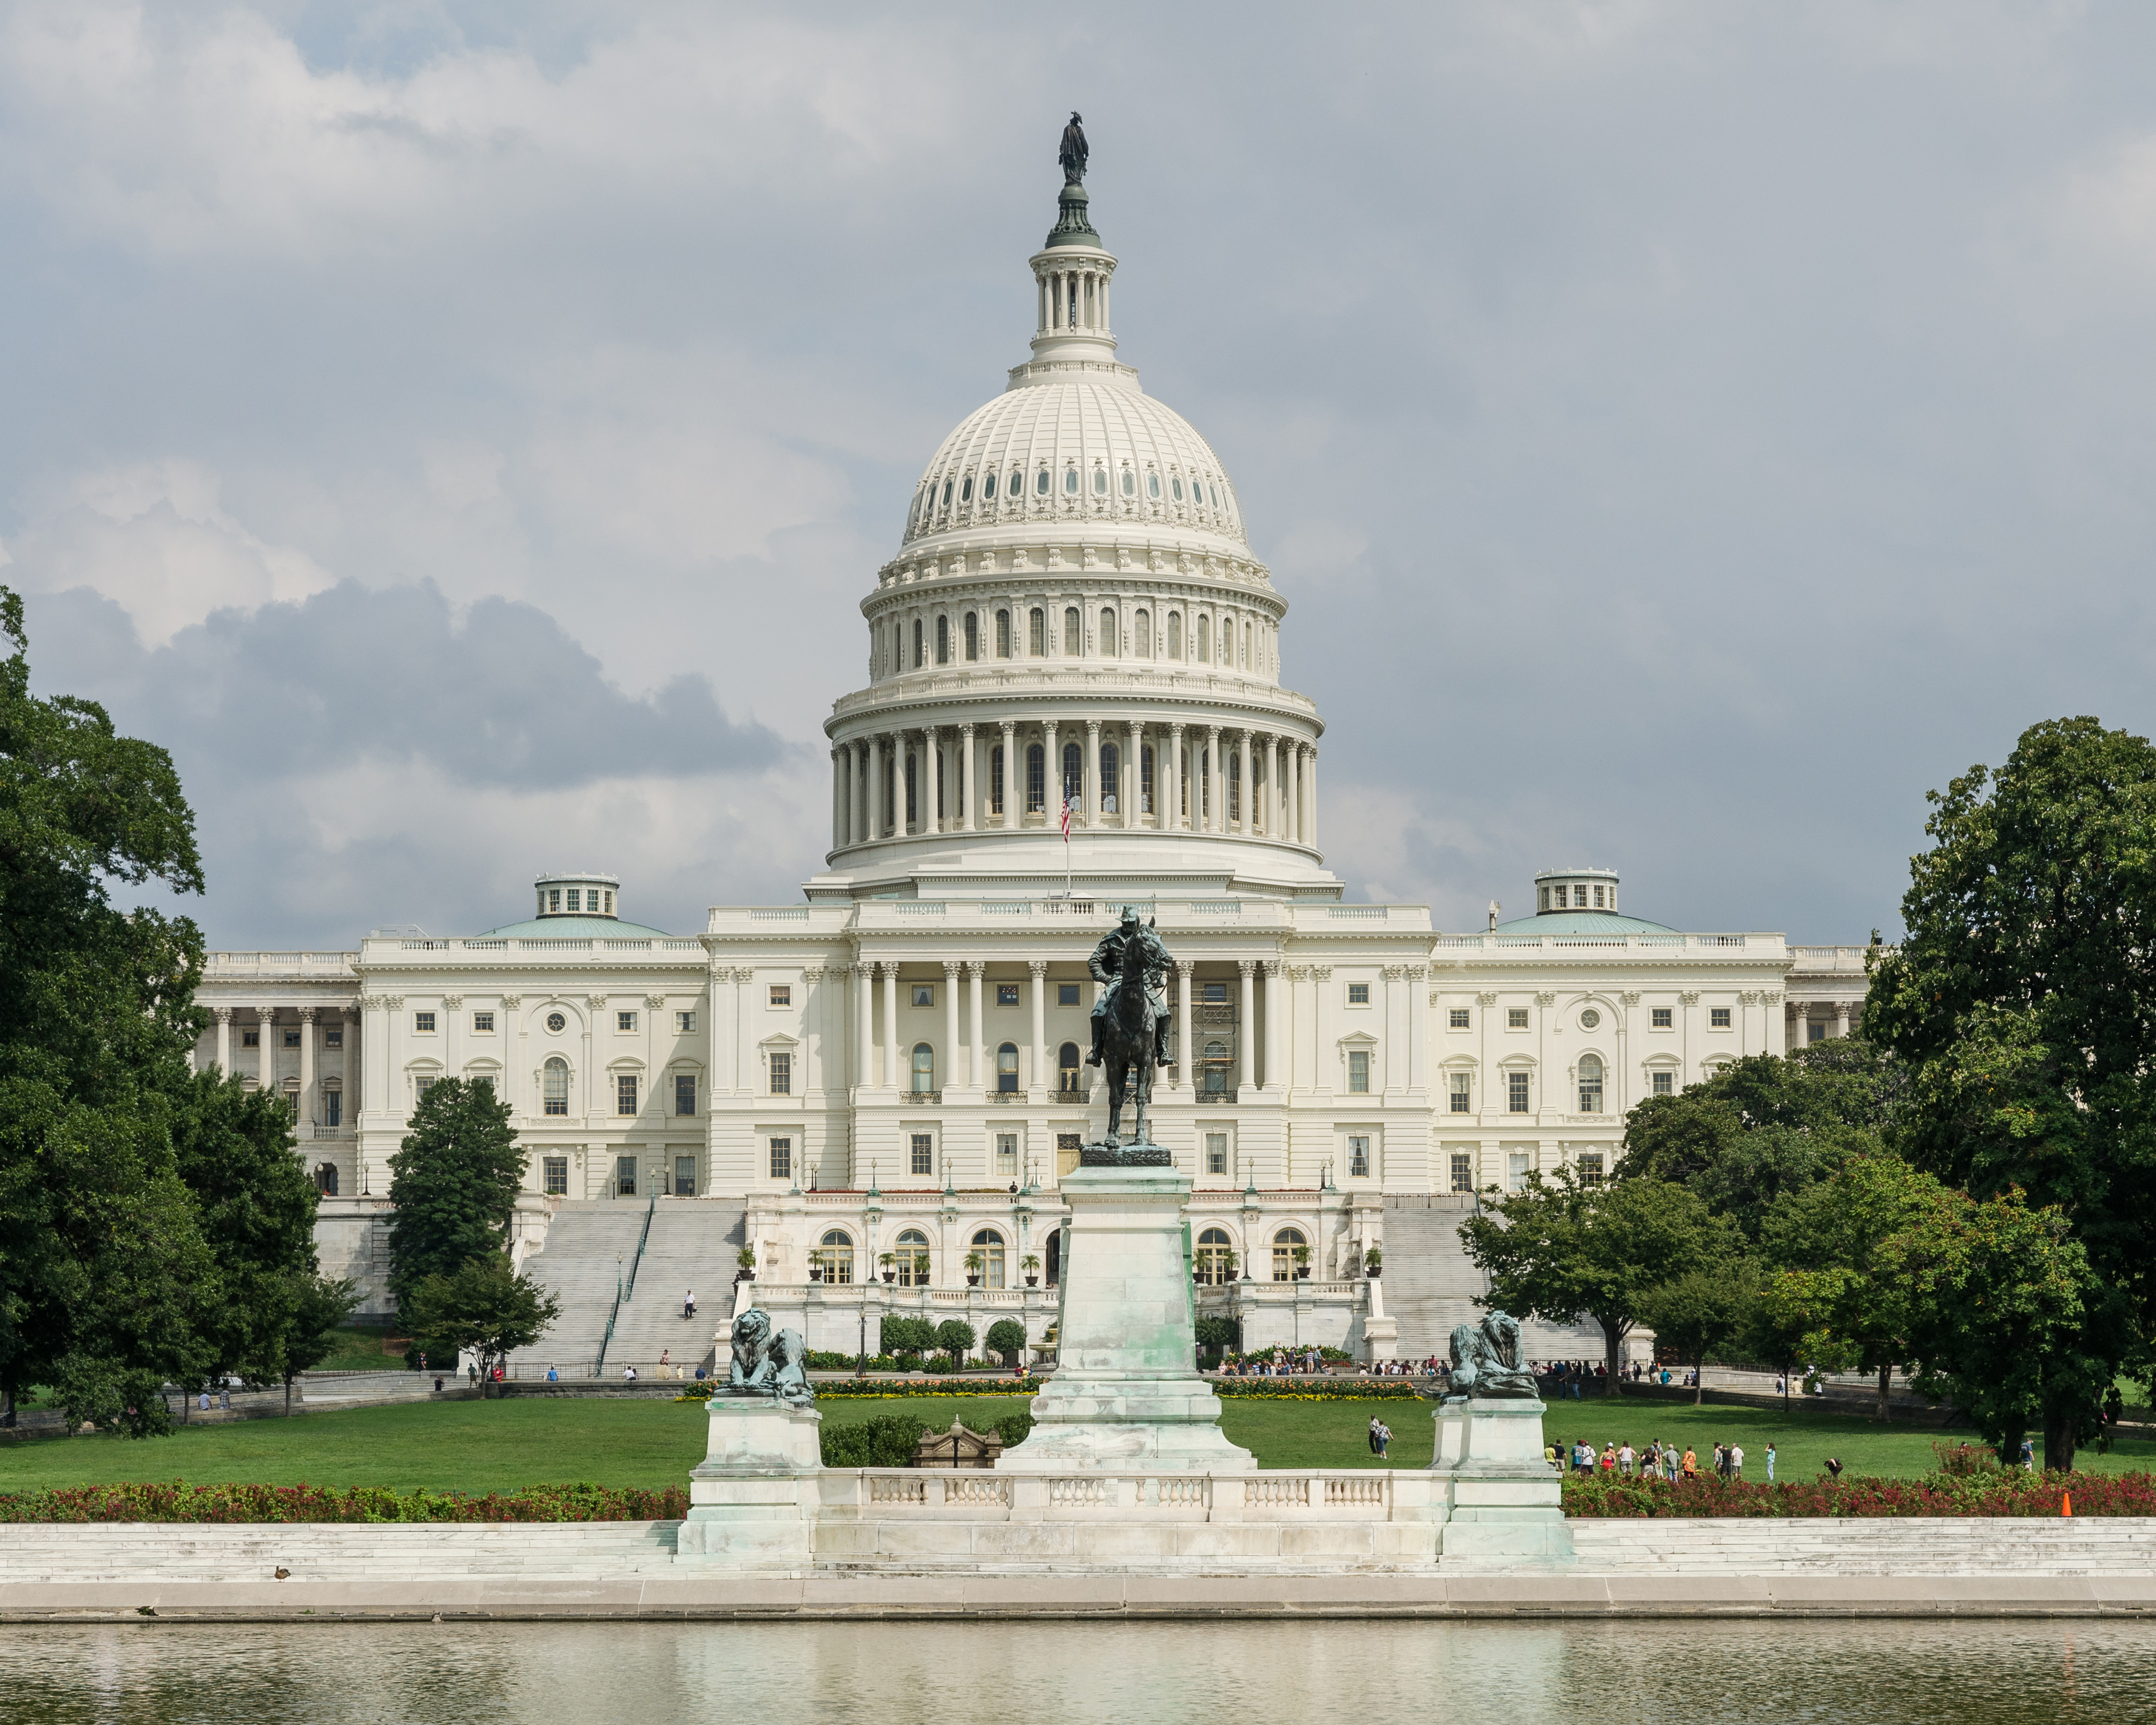
\includegraphics[width=\linewidth]{images/dc/dc_capitol.jpg}
\end{minipage}

\vspace{0.3em}
\noindent
\begin{minipage}[t]{0.48\textwidth}
  
\includegraphics[width=\linewidth]{images/dc/dc_cherry_blossoms.jpg}
\end{minipage}\hfill
\begin{minipage}[t]{0.48\textwidth}
  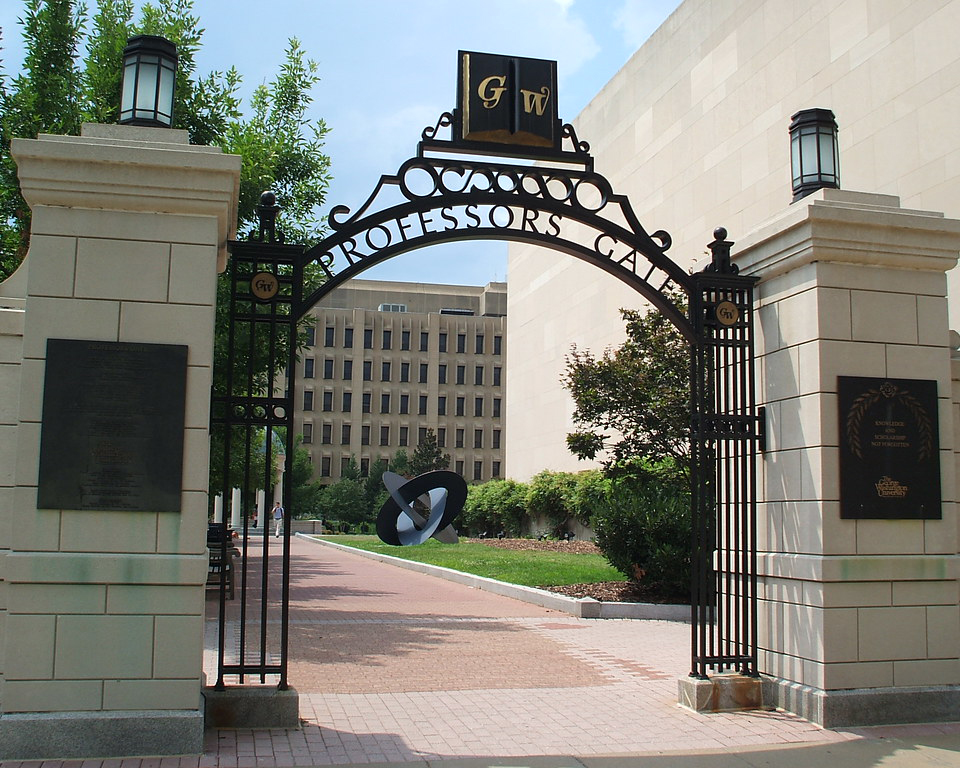
\includegraphics[width=\linewidth]{images/dc/gwu_kogan_plaza.jpg}
\end{minipage}

\newpage

\thispagestyle{empty}
\markboth{}{}
\begin{center}
{\Large\textbf{WELCOME}}
\end{center}
\vspace{0.5em}
\noindent\textbf{\large John Gray, President of the Industry Studies Association}

\vspace{1em}
\noindent [PLACEHOLDER: Insert president's message text here.]

\vspace{2em}
\noindent John Gray\\
President, ISA

\vspace{1.5em}
\begin{center}
  
\includegraphics[width=0.35\textwidth]{images/john-gray.png}
\end{center}
\newpage

\thispagestyle{empty}
\markboth{}{}
\begin{center}
  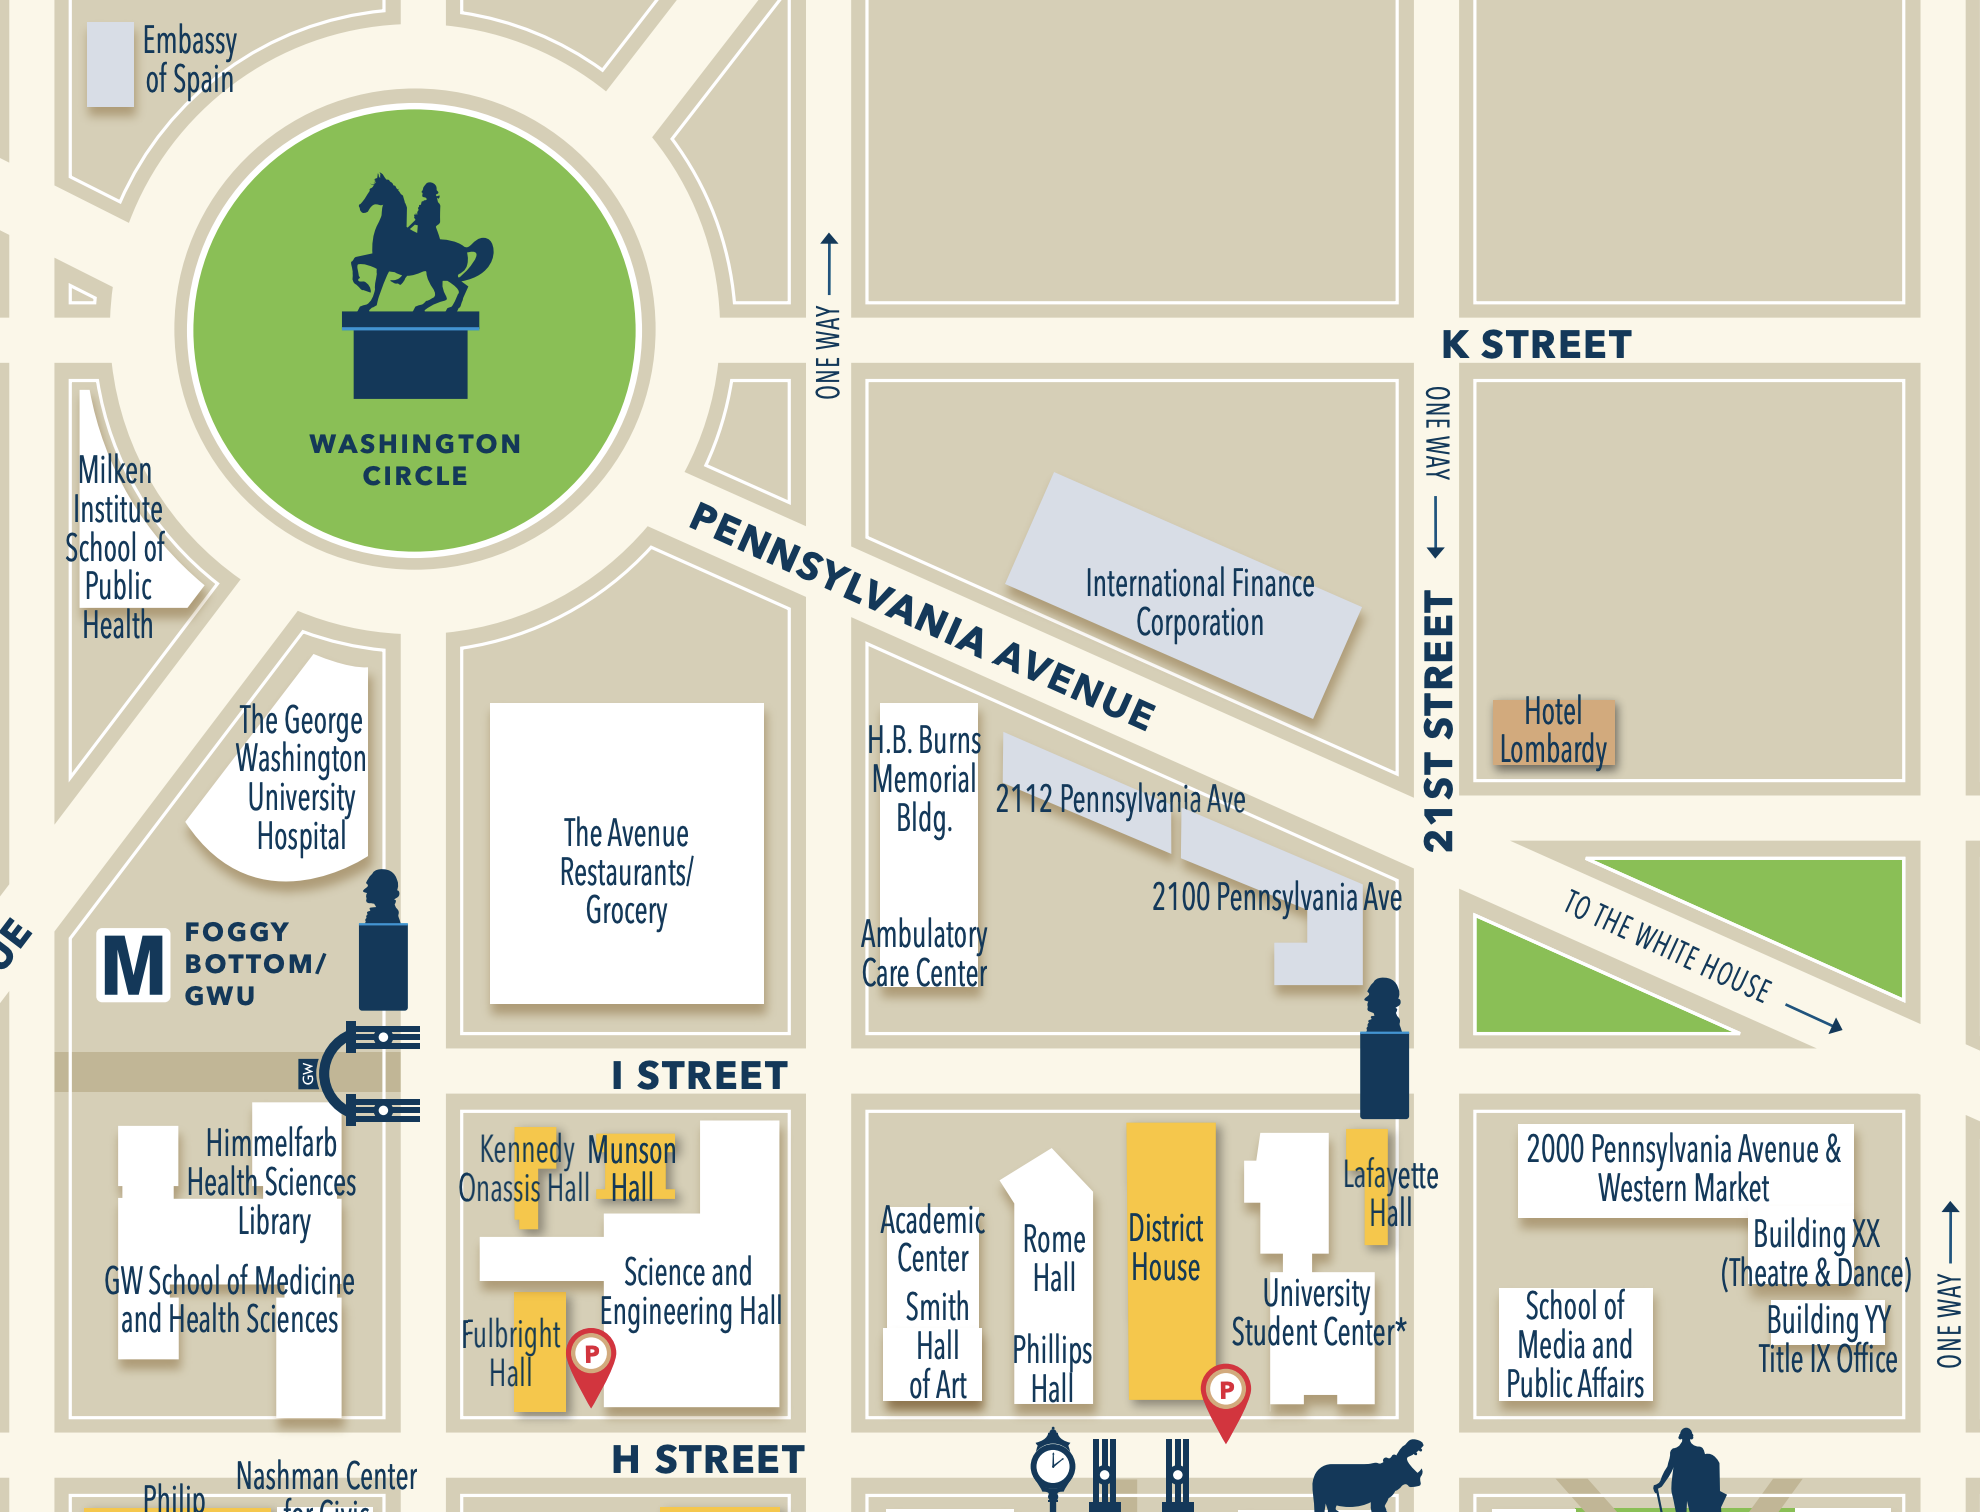
\includegraphics[width=\textwidth, height=\textheight, keepaspectratio]{images/map.png}
\end{center}
\newpage

\markboth{}{}
\noindent\textbf{\Large ISA 2026 Award Winners}\par
\vspace{0.5em}
{\small
\noindent\textcolor{event}{\textbf{BEST PAPER IN INNOVATION AND ENTREPRENEURSHIP}}\par\vspace{0.1em}
\noindent\textit{This award recognizes outstanding innovation and entrepreneurship research. Papers from any research stream are eligible, including self-nominations. Winning papers must demonstrate significant personal investment in understanding industry-specific markets, firms, and institutions, typically integrating field-based research with appropriate theory and analysis, aligning with the Industry Studies Association's mission. Prizes: \$500 (first place), \$250 (runner-up).}\par\vspace{0.15em}
\noindent \textbf{Winner:} \textit{``Mind the Gap in Drug Development: Understanding the Whitespace Between Clinical Trials''}\par
\noindent Sukhun Kang (UC Santa Barbara); Sandra Barbosu (New York University); Fan Ye (UC Santa Barbara); Sungyong Chang (Cornell University)\par
\vspace{0.2em}

\noindent \textbf{Runner-up:} \textit{``Misleading Science Maps: Firms' Strategic Responses to Data Malpractice in Alzheimer's Research''}\par
\noindent Matteo Tranchero (The Wharton School); Christian Fons-Rosen (UC Merced); Lee Fleming (UC Berkeley)\par
\vspace{0.2em}

\noindent\textbf{Award Committee:} John Paul Helveston\par
\vspace{0.4em}

\noindent\textcolor{event}{\textbf{BABBAGE BEST PAPER IN INDUSTRIAL INNOVATION POLICY}}\par\vspace{0.1em}
\noindent\textit{This new award, funded by the Babbage International Policy Forum (UK) under Professor Sir Mike Gregory's leadership, recognizes outstanding contributions to industrial innovation policy research. Winning papers must demonstrate deep engagement with theoretical and practical elements of industrial innovation policy and substantial commitment to understanding policy-industry dynamics. Cross-disciplinary approaches drawing from economics, science and technology, and management are encouraged, particularly those offering practical insights for policymakers and industry leaders. Prizes: \$750 (first place), \$250 (runner-up).}\par\vspace{0.15em}
\noindent \textbf{Winner:} \textit{``Implementing a Comprehensive Intervention to Promote Sustainable Agricultural Practices in India''}\par
\noindent Subhankar Saha (Ahmedabad University, India); Haritha Saranga (Indian Institute of Management Bangalore, India); Sriram Narayanan (Michigan State University); Chandrakant Pradhan (Confederation of Indian Industry, India)\par
\vspace{0.2em}

\noindent \textbf{Runner-up:} \textit{``Data Privacy Regulation and Innovation''}\par
\noindent Sukhun Kang (University of California Santa Barbara); Jennifer Kao (University of California Los Angeles)\par
\vspace{0.2em}

\noindent\textbf{Award Committee:} John Paul Helveston\par
\vspace{0.4em}

\noindent\textcolor{event}{\textbf{GIARRATANI RISING STAR AWARD}}\par\vspace{0.1em}
\noindent\textit{Early career scholars may submit one paper to which they've made a significant contribution. This award recognizes junior scholars conducting industry-based research that demonstrates deep knowledge through significant personal investment in understanding industry markets, firms, and institutions. Prizes: \$1,000 (first place), \$500 (runner-up).}\par\vspace{0.15em}
\noindent \textbf{Winner:} \textit{``Dynamic Competition in Networked Markets: Evidence from US Broadband''}\par
\noindent Jennifer Zou (Harvard University)\par
\vspace{0.2em}

\noindent \textbf{Runner-up:} \textit{``Offshore Manufacturing of Innovative Drugs: Evidence from U.S. Pharmaceutical Firms''}\par
\noindent Minji Lee (Cornell University)\par
\vspace{0.2em}

\noindent\textbf{Award Committee:} John Paul Helveston\par
\vspace{0.4em}

\noindent\textcolor{event}{\textbf{RALPH GOMORY BEST INDUSTRY STUDIES PAPER AWARD}}\par\vspace{0.1em}
\noindent\textit{Named for Ralph Gomory, former Alfred P. Sloan Foundation President who initiated the Industry Studies Program, this award showcases excellent industry studies research published in the preceding year across eight top academic journals. The Industry Studies Association aims to encourage researchers to submit industry studies work to leading scholarly journals while demonstrating to editors the value of deep industry context exploration. The ISA promotes research that builds practitioner relationships for primary data access, uses field-gathered contextual knowledge to inform research questions and design, and guides data analysis, interpretations, and conclusions. Prizes: \$1,000 (first place), \$500 (runner-up).}\par\vspace{0.15em}
\noindent \textbf{Winner:} \textit{``Contradictory control: How employers' multiple control practices clash and enable workers' acts of resistance''}\par
\noindent Yuequan Guo (WZB Berlin Social Science Center)\par
\noindent\textit{ILR Review, 78(5), 780–805. https://doi.org/10.1177/00197939251357273}\par
\vspace{0.2em}

\noindent \textbf{Runner-up:} \textit{``The perils of a soft start: Initial conditions''}\par
\noindent early strategy selection\par
\noindent\textit{and small firm performance. F. Christopher Eaglin (Fuqua School of Business, Duke University)}\par
\noindent\textit{Dissertation Committee: Strategic Management Journal, 46(9), 2113–2165}\par
\vspace{0.2em}

\noindent\textbf{Award Committee:} John Paul Helveston\par
\vspace{0.4em}

\noindent\textcolor{event}{\textbf{DISSERTATION AWARD}}\par\vspace{0.1em}
\noindent\textit{This award recognizes outstanding doctoral research in industry studies. Eligible candidates must have completed a dissertation in economics, management, engineering, political science, sociology, or related/interdisciplinary fields within the previous 18 months. Prizes: \$500 (first place), \$250 (runner-up).}\par\vspace{0.15em}
\noindent \textbf{Winner:} \textit{``Coevolution of Small Business Strategy and Regulation: A Mixed-Methods Study of United States Craft Breweries''}\par
\noindent Eppa Rixey (MIT-Sloan, currently Northeastern University)\par
\noindent\textit{Dissertation Committee: Susan Silbey (Chair); Ezra Zuckerman Sivan; Stine Grodal; Johan Chu}\par
\vspace{0.2em}

\noindent \textbf{Runner-up:} \textit{``The Role of Data in the Search for Innovation: Essays on Big Data Genomics''}\par
\noindent Matteo Tranchero (UC Berkeley, currently The Wharton School)\par
\noindent\textit{Dissertation Committee: Abhishek Nagaraj (Co-Chair); Lee Fleming (Co-Chair); Toby Stuart; Carolyn Stein; Enrico Moretti}\par
\vspace{0.2em}

\noindent\textbf{Award Committee:} John Paul Helveston\par
\vspace{1.5em}

\begin{center}\textbf{Join us Friday, June 6th at the awards luncheon, when we will recognize all awardees.}\end{center}
}
\newpage

\markboth{}{}
\noindent\textbf{\Large Conference in Brief}\par\vspace{0.5em}
{\renewcommand{\arraystretch}{0.9}
\noindent\textcolor{event}{\textbf{REGISTRATION}}\par\vspace{0.15em}
\begin{tabular}{@{}p{3.2cm}p{\dimexpr\linewidth-3.5cm}@{}}
  Wed., June 3 & 8:00am--6:00pm\quad Science \& Engineering Hall, B1 \\
  Wed., June 3 & 11:30am--2:00pm\quad Milken Institute \\
  Thu.--Fri., June 4--5 & Student Center, 3rd Floor \\
\end{tabular}

\vspace{0.5em}
\noindent\textcolor{event}{\textbf{WEDNESDAY, June 3}}\par\vspace{0.15em}
\begin{tabular}{@{}p{3.2cm}p{\dimexpr\linewidth-3.5cm}@{}}
  \multicolumn{2}{@{}l@{}}{\textbf{Science \& Engineering Hall}} \\
  8:00am--11:30am & Morning Excursion Option 1: Intro to DC non profits \\
  \multicolumn{2}{@{}l@{}}{\textbf{Lincoln Memorial}} \\
  8:00am--11:30am & Morning Excursion Option 2: DC Mall Tour \\
  \multicolumn{2}{@{}l@{}}{\textbf{Milkin Institute}} \\
  12:00pm--1:00pm & Lunch \\
  1:00pm--1:55pm & \textcolor{event}{Opening Plenary} \\
  2:00pm--4:40pm & \textcolor{event}{PDW} \\
  \multicolumn{2}{@{}l@{}}{\textbf{Science \& Engineering Hall}} \\
  2:00pm--3:10pm & \textcolor{event}{Paper Sessions} \\
  3:10pm--3:30pm & Break \\
  3:30pm--4:40pm & \textcolor{event}{Paper Sessions} \\
  4:45pm--5:55pm & \textcolor{event}{Paper Sessions} \\
  6:00pm--7:00pm & Reception \\
\end{tabular}

\vspace{0.5em}
\noindent\textcolor{event}{\textbf{THURSDAY, June 4}}\par\vspace{0.15em}
\begin{tabular}{@{}p{3.2cm}p{\dimexpr\linewidth-3.5cm}@{}}
  \multicolumn{2}{@{}l@{}}{\textbf{Student Center}} \\
  8:20am--9:00am & Breakfast \\
  9:00am--10:10am & \textcolor{event}{Paper Sessions} \\
  10:10am--10:40am & Break \\
  10:40am--11:40am & \textcolor{event}{Concurrent Panel Sessions} \\
  11:40am--12:45pm & Lunch \& Business Meeting \\
  12:50pm--2:00pm & \textcolor{event}{Paper Sessions} \\
  2:05pm--3:05pm & \textcolor{event}{Concurrent Panel Sessions} \\
  3:05pm--3:35pm & Break \\
  3:40pm--4:50pm & \textcolor{event}{Paper Sessions} \\
  4:55pm--6:00pm & \textcolor{event}{Concurrent Panel Sessions} \\
  6:00pm--8:00pm & Reception \\
\end{tabular}

\vspace{0.5em}
\noindent\textcolor{event}{\textbf{FRIDAY, June 5}}\par\vspace{0.15em}
\begin{tabular}{@{}p{3.2cm}p{\dimexpr\linewidth-3.5cm}@{}}
  \multicolumn{2}{@{}l@{}}{\textbf{Student Center}} \\
  8:20am--9:00am & Breakfast \\
  9:00am--10:00am & \textcolor{event}{Concurrent Panel Sessions} \\
  10:00am--10:30am & Break \\
  10:30am--11:40am & \textcolor{event}{Paper Sessions} \\
  11:40am--12:40pm & Lunch \& Awards Ceremony \\
\end{tabular}
}
\newpage

\markboth{}{}
\noindent\textbf{\large Research stream descriptions, abbreviations, and color key:}

\vspace{1.2em}

\noindent\textbf{\textcolor{sustainability}{1. Energy, Sustainable Innovation, and Mobility (EN)}}

\vspace{0.3em}
\noindent This stream invites papers and panels on the changing market and public policy landscape where the energy industry (including oil and gas, electricity, pipelines) intersects with environmental concerns.

\vspace{1em}

\noindent\textbf{\textcolor{gis}{2. General Industry Studies (GO)}}

\vspace{0.3em}
\noindent Any research on issues or industries not covered in other research streams described above may be submitted to this general stream. Papers or organized panels comparing phenomena, trends, issues, or economic activities across occupations, industries, or geographic regions are especially welcome.

\vspace{1em}

\noindent\textbf{\textcolor{health}{3. Health Care Systems, Biotechnology, and Pharmaceuticals (HC)}}

\vspace{0.3em}
\noindent This stream invites papers and panels that examine the myriad of issues surrounding effective management of health care entities and systems (e.g., hospitals, medical groups, public health agencies, insurance companies, pharmaceutical firms, technology companies, etc.).

\vspace{1em}

\noindent\textbf{\textcolor{innovation}{4. Innovation, Entrepreneurship, and AI-Driven Transformation (IE)}}

\vspace{0.3em}
\noindent This stream invites papers and panels that examine innovation within firms and other organizations such as universities, across organizational boundaries, across country boundaries, and in new entrepreneurial ventures.

\vspace{1em}

\noindent\textbf{\textcolor{labor}{5. Labor Markets, Organizations, and the Future of Work (LM)}}

\vspace{0.3em}
\noindent This stream welcomes papers and panels that examine the impacts of firm, industry, and market characteristics on labor markets, industrial relations, and/or human resource practices as well as public policy outcomes.

\vspace{1em}

\noindent\textbf{\textcolor{operations}{6. Operations, Supply Chain, and AI-Enhanced Industry 4.0 (OP)}}

\vspace{0.3em}
\noindent This stream welcomes papers and panels that are concerned with the oversight, design, and control of the business processes responsible for the production of goods and services as well as those focused on coordination of (multiple) firms responsible for these business processes within a supply network.

\vspace{1em}

\noindent\textbf{\textcolor{policy}{7. Public Policy, and Global Competitiveness (PP)}}

\vspace{0.3em}
\noindent Public policy -- whether national, regional, local or global -- often shapes opportunities for industries, including competitive options within industries and globalization of industries. In turn, wrestling with these opportunities, competitiveness and globalization have had a profound impact on the nature of industrial activity and policy.

\newpage

\markboth{}{}
\noindent\colorbox{event}{\parbox{\dimexpr\linewidth-2\fboxsep}{\centering\textcolor{white}{\large\textbf{Conference Program: Wednesday, June 3}}}}

\vspace{0.6em}

{\renewcommand{\arraystretch}{0.9}

\noindent\textcolor{event}{\textbf{MORNING EXCURSION OPTION 1: INTRO TO DC NON PROFITS}}

\begin{tabular}{@{}p{3.2cm}p{\dimexpr\linewidth-3.5cm}@{}}
  8:00am--11:30am & Science \& Engineering Hall, B1 1270 \\
\end{tabular}

\vspace{0.25em}

\noindent\textcolor{event}{\textbf{MORNING EXCURSION OPTION 2: DC MALL TOUR}}

\begin{tabular}{@{}p{3.2cm}p{\dimexpr\linewidth-3.5cm}@{}}
  8:00am--11:30am & Lincoln Memorial \\
\end{tabular}

\vspace{0.25em}

\noindent\textcolor{event}{\textbf{LUNCH}}

\begin{tabular}{@{}p{3.2cm}p{\dimexpr\linewidth-3.5cm}@{}}
  12:00pm--1:00pm & Milkin Institute, Convening Hall \\
\end{tabular}

\vspace{0.25em}

\noindent\textcolor{event}{\textbf{OPENING PLENARY}}

\begin{tabular}{@{}p{3.2cm}p{\dimexpr\linewidth-3.5cm}@{}}
  1:00pm--1:55pm & Milkin Institute, Convening Hall \\
\end{tabular}

\vspace{0.25em}

\noindent\textcolor{event}{\textbf{PDW}}

\begin{tabular}{@{}p{3.2cm}p{\dimexpr\linewidth-3.5cm}@{}}
  2:00pm--4:40pm & Milkin Institute, Convening Hall \\
\end{tabular}

\vspace{0.25em}

\noindent\textcolor{event}{\textbf{PAPER SESSIONS}}

\begin{tabular}{@{}p{3.2cm}p{\dimexpr\linewidth-3.5cm}@{}}
  2:00pm--3:10pm & Science \& Engineering Hall, Classrooms \\
\end{tabular}

\vspace{0.25em}

\noindent\textcolor{event}{\textbf{BREAK}}

\begin{tabular}{@{}p{3.2cm}p{\dimexpr\linewidth-3.5cm}@{}}
  3:10pm--3:30pm & Science \& Engineering Hall, B1 Greenwall \\
\end{tabular}

\vspace{0.25em}

\noindent\textcolor{event}{\textbf{PAPER SESSIONS}}

\begin{tabular}{@{}p{3.2cm}p{\dimexpr\linewidth-3.5cm}@{}}
  3:30pm--4:40pm & Science \& Engineering Hall, Classrooms \\
\end{tabular}

\vspace{0.25em}

\noindent\textcolor{event}{\textbf{PAPER SESSIONS}}

\begin{tabular}{@{}p{3.2cm}p{\dimexpr\linewidth-3.5cm}@{}}
  4:45pm--5:55pm & Science \& Engineering Hall, Classrooms \\
\end{tabular}

\vspace{0.25em}

\noindent\textcolor{event}{\textbf{RECEPTION}}

\begin{tabular}{@{}p{3.2cm}p{\dimexpr\linewidth-3.5cm}@{}}
  6:00pm--7:00pm & Science \& Engineering Hall, B1 Greenwall \\
\end{tabular}

\vspace{0.25em}

}
\newpage

\markboth{Wednesday, June 3}{Morning Excursion Option 1: Intro to DC non profits}

\begin{center}
\colorbox{event!15}{\parbox{0.9\linewidth}{\centering
  \textcolor{event}{\large\textbf{Morning Excursion Option 1: Intro to DC non profits}}\\[2pt]
  {\small Wednesday, 08:00 AM – 11:30 AM $\cdot$ \textit{Science \& Engineering Hall, B1 1270}}
}}
\end{center}

\vspace{1em}

\markboth{Wednesday, June 3}{Morning Excursion Option 2: DC Mall Tour}

\begin{center}
\colorbox{event!15}{\parbox{0.9\linewidth}{\centering
  \textcolor{event}{\large\textbf{Morning Excursion Option 2: DC Mall Tour}}\\[2pt]
  {\small Wednesday, 08:00 AM – 11:30 AM $\cdot$ \textit{Lincoln Memorial, NA}}
}}
\end{center}

\vspace{1em}

\markboth{Wednesday, June 3}{Lunch}

\begin{center}
\colorbox{event!15}{\parbox{0.9\linewidth}{\centering
  \textcolor{event}{\large\textbf{Lunch}}\\[2pt]
  {\small Wednesday, 12:00 PM – 01:00 PM $\cdot$ \textit{Milkin Institute, Convening Hall}}
}}
\end{center}

\vspace{1em}

\markboth{Wednesday, June 3}{Plenary Session | 01:00 PM – 02:00 PM}

\begin{center}
\normalsize\textit{Plenary Session}\\[0.3em]
\Large\textbf{Wednesday, 01:00 PM – 02:00 PM}
\end{center}

\subsection{\texorpdfstring{\textcolor{policy}{Public Policy and Global Competitiveness}}{}}\label{section}

\textbf{Fireside Chat: Dr.~Laura Taylor-Kale \& Dr.~Monica Gorman}
\emph{(Panel Discussion)} --- Room Milken - Convening Hall

\textbf{Panelists:}

\begin{itemize}
\tightlist
\item
  Dr.~Monica Gorman (Managing Director, Crowell Global Advisors)
\item
  Dr.~Laura Taylor-Kale (Senior Fellow for Geoeconomics and Defense at
  the Council on Foreign Relations)
\end{itemize}

In this fireside chat, two leading voices on industrial policy and
economic security will explore the challenges and opportunities facing
America's industrial base in an era of intensifying geopolitical
competition. Dr.~Monica Gorman, Managing Director at Crowell Global
Advisors, brings over two decades of experience spanning both the public
and private sectors --- most recently serving as Special Assistant to
the President for Manufacturing and Industrial Policy at the White House
National Economic Council, where she spearheaded the establishment of
the White House Council on Supply Chain Resilience and led the nation's
Supply Chain Disruptions Task Force. Before her government service,
Dr.~Gorman spent nine years as Vice President of Responsible Leadership
and Global Compliance at New Balance, giving her a rare ground-level
perspective on how trade policy, tariffs, and supply chain risk play out
in practice for U.S. manufacturers. She will be joined by Dr.~Laura
Taylor-Kale, Senior Fellow for Geoeconomics and Defense at the Council
on Foreign Relations, who served as the first presidentially-appointed,
Senate-confirmed Assistant Secretary of Defense for Industrial Base
Policy from 2023 to 2025 --- a role in which she led all defense
industrial strategy and investments and authored the Pentagon's
first-ever National Defense Industrial Strategy. Together, they bring a
powerful combination of White House, Pentagon, Commerce Department, and
private sector experience to bear on the defining industrial policy
questions of our time.

\vspace{1em}

\markboth{Wednesday, June 3}{PDW}

\begin{center}
\colorbox{event!15}{\parbox{0.9\linewidth}{\centering
  \textcolor{event}{\large\textbf{PDW}}\\[2pt]
  {\small Wednesday, 02:00 PM – 04:40 PM $\cdot$ \textit{Milkin Institute, Convening Hall}}
}}
\end{center}

\newpage

\markboth{Wednesday, June 3}{Paper Sessions | 02:00 PM – 03:10 PM}

\begin{center}
\normalsize\textit{Paper Sessions}\\[0.3em]
\Large\textbf{Wednesday, 02:00 PM – 03:10 PM}
\end{center}

\subsection{\texorpdfstring{\textcolor{health}{Health Care Systems, Biotechnology, and Pharmaceuticals}}{}}\label{section-1}

\textbf{Drug Pricing and Market Competition} --- Room SEH-1400

\textbf{Session Chair:} Miguel Sanchez (Johns Hopkins University)

\begin{enumerate}
\def\labelenumi{\arabic{enumi}.}
\item
  \textbf{Miguel Sanchez (Johns Hopkins University); Antonio Trujillo
  (Johns Hopkins Bloomberg School of Public Health); Manuel Hermosilla
  (University of Illinois Chicago); So-Yeon Kang (Georgetown School of
  Health); Jason Gibbons (Brigham and Women's Hospital/Harvard Medical
  School)} --- Drug Coupons as a Strategic Lever: Expanding Access or a
  Brand Loyalty Acquisition Tool?
\item
  \textbf{Morgane Mouslim (University of Michigan ); Jeffrey Mccullough
  (University of Michigan); Antonio Trujillo (Johns Hopkins University
  )} --- Market Size, Biosimilar Entry, and Price Competition in U.s.
  Biologic Drug Markets
\item
  \textbf{Mariana Socal (Johns Hopkins Bloomberg School of Public
  Health); Yunxiang Sun (Johns Hopkins Bloomberg School of Public
  Health); Jeromie Ballreich (Johns Hopkins Bloomberg School of Public
  Health); Joy Acha (Johns Hopkins Bloomberg School of Public Health);
  Mohammad Ali Yazdi (Johns Hopkins Carey Business School); Tinglong Dai
  (Johns Hopkins Carey Business School); Maqbool Dada (Johns Hopkins
  Carey Business School)} --- Potential Impact of Tariffs on the Price
  of Generic Drugs Made in the Us with Imported Active Ingredients
\item
  \textbf{Allison Kim (Georgetown University); So-Yeon Kang (Georgetown
  University)} --- Global Availability and Prices of Medicare's
  Ultra-Expensive Drugs: Implications for a Most Favored Nation Policy
\end{enumerate}

\subsection{\texorpdfstring{\textcolor{innovation}{Innovation, Entrepreneurship, and AI-Driven Transformation}}{}}\label{section-2}

\textbf{Technology Legitimacy and Emerging Markets} --- Room SEH-1450

\textbf{Session Chair:} Scott Taylor (University of Southern California)

\begin{enumerate}
\def\labelenumi{\arabic{enumi}.}
\item
  \textbf{Scott Taylor (University of Southern California)} --- Latent
  Hazards: Counterperformative Effects of Certification in New Ventures
\item
  \textbf{Rui Wang (Tsinghua University); Joel Gehman (George Washington
  University)} --- Multimodal Optimal Distinctiveness
\item
  \textbf{Rohit Verma (University of South Carolina), Kejia Hu
  (University of Oxford), Xin Ding (Rutgers University), and Diep Pham
  (University of South Carolina)} --- Service Design and Innovation for
  Aging Societies: Introducing Silver Prosperity Index (Spi)
\end{enumerate}

\subsection{\texorpdfstring{\textcolor{labor}{Labor Markets, Organizations, and the Future of Work}}{}}\label{section-3}

\textbf{Organizational Structure and Human Capital} --- Room SEH-3040

\textbf{Session Chair:} Alan Zhang (Columbia)

\begin{enumerate}
\def\labelenumi{\arabic{enumi}.}
\item
  \textbf{Alan Zhang (Columbia)} --- Jurisdictional Decoupling: When
  Service Providers Expand Control by Distancing Other Groups from Their
  Work
\item
  \textbf{Manuel Torres-Sahli (Universidad De Los Andes, Chile); Alfredo
  Enrione (Ese Business School, Universidad De Los Andes, Chile);
  Santiago Truffa (Universidad Adolfo Ibañez, Chile); Felipe Aldunate
  (Ese Business School, Universidad De Los Andes, Chile); Jacinta
  Girardi (Buk, Chile); Constanza Opazo (Buk, Chile)} --- Hierarchies:
  New Facts from Administrative Hr Data
\item
  \textbf{Junseok Goh (University of Wisconsin - Madison)} --- Do
  Managers Capture Firm Surplus? Evidence from Human Capital Development
  and Residual Profits
\end{enumerate}

\subsection{\texorpdfstring{\textcolor{operations}{Operations, Supply Chain, and AI-Enhanced Industry 4.0}}{}}\label{section-4}

\textbf{Digital Technology in Manufacturing} --- Room SEH-1300

\textbf{Session Chair:} Ilkim Güneri (ETH Zurich)

\begin{enumerate}
\def\labelenumi{\arabic{enumi}.}
\item
  \textbf{Ilkim Güneri (ETH Zurich); Oliver Von Dzengelevski (ETH
  Zurich); John Gray (The Ohio State University); Torbjorn Netland (ETH
  Zurich)} --- Learning Curve Effects in Outsourcing: Evidence from the
  Medtech Industry
\item
  \textbf{Tianyu Xu (The Ohio State University); Xiang Wan (The Ohio
  State University)} --- Cascading Failures: an Analysis of a Major It
  Outage
\item
  \textbf{Mehreen Tahir (University of Camerino)} --- Is Blockchain a
  One-Size-Fits-All Innovation for Agriculture? Evidence from a
  Systematic Review Across Ecosystem Domains
\item
  \textbf{Adamu Jaafaru (Metro State University)} --- Digital Twin
  Adoption and Sustainability Outcomes in Manufacturing: an Industry
  Capability Perspective
\end{enumerate}

\subsection{\texorpdfstring{\textcolor{policy}{Public Policy and Global Competitiveness}}{}}\label{section-5}

\textbf{Technology Competitiveness and National Security} --- Room
SEH-B1220

\textbf{Session Chair:} Angela Garcia Calvo (University of Reading)

\begin{enumerate}
\def\labelenumi{\arabic{enumi}.}
\item
  \textbf{Angela Garcia Calvo (University of Reading)} --- Does the
  Transition to Battery Electric, Software-Defined Vehicles Create
  Opportunities for Europe?
\item
  \textbf{Max Walter (Akili Economic Development)} --- Industrial
  Statecraft in the New Global Order: a Survival Guide for Lmics
\item
  \textbf{Prathyaj Mantha (PEER Consultants, P.C.)} --- The Real
  Bottleneck in Ai: Power Generation, Environmental Policy, and National
  Competitiveness
\end{enumerate}

\subsection{\texorpdfstring{\textcolor{sustainability}{Sustainable Innovation, Energy, and Mobility}}{}}\label{section-6}

\textbf{Taking Stock: System Dynamics Modeling in Industry Studies} ---
Room SEH-B1270

\textbf{Session Chair:} Sergey Naumov (Pennsylvania State University)

\begin{enumerate}
\def\labelenumi{\arabic{enumi}.}
\item
  \textbf{Sergey Naumov (Pennsylvania State University)} --- Managing
  Capacity for Electric Vehicle Batteries Recycling
\item
  \textbf{Edward Anderson (University of Texas at Austin), Sergey Naumov
  (Pennsylvania State University), Burcu Tan (University of New Mexico),
  Robert Benny (University of Texas at Austin)} --- Cartels, Policy, and
  Technological Substitution: What the History of the Synthetic Rubber
  Industry Can Teach Us About the Rare Earths Supply Chain
\item
  \textbf{Alexander Kuptel (MIT Sloan School of Management), John
  Sterman (MIT Sloan School of Management)} --- Doubling Down on
  Dual-Fuels: Heat Pump and Fossil Backups' Effects on Grid Load, Cost,
  and Emissions in Massachusetts
\item
  \textbf{Nikolai Kazantsev (University of Cambridge), Ettore Settanni
  (University of Cambridge), Jagjit Singh Srai (University of
  Cambridge)} --- The Role of Public Infrastructure in Food Systems
  Resilience: a Model-Based Strategy to Revitalise Wholesale Markets
\end{enumerate}

\vspace{1em}

\markboth{Wednesday, June 3}{Break}

\begin{center}
\colorbox{event!15}{\parbox{0.9\linewidth}{\centering
  \textcolor{event}{\large\textbf{Break}}\\[2pt]
  {\small Wednesday, 03:10 PM – 03:30 PM $\cdot$ \textit{Science \& Engineering Hall, B1 Greenwall}}
}}
\end{center}

\vspace{1em}

\markboth{Wednesday, June 3}{Paper Sessions | 03:30 PM – 04:40 PM}

\begin{center}
\normalsize\textit{Paper Sessions}\\[0.3em]
\Large\textbf{Wednesday, 03:30 PM – 04:40 PM}
\end{center}

\subsection{\texorpdfstring{\textcolor{gis}{General Industry Studies}}{}}\label{section-7}

\textbf{Industrial Policy and Market Governance} --- Room SEH-1450

\textbf{Session Chair:} Audrey Stienon (Open Markets Institute)

\begin{enumerate}
\def\labelenumi{\arabic{enumi}.}
\item
  \textbf{Audrey Stienon (Open Markets Institute)} --- Coordinating
  Market Actors for the Public Good: Competition Policy as the
  Industrial Policy of Democratic Economic Governance
\item
  \textbf{Alexander Bendel (University of Duisburg-Essen); Thomas Bendel
  (University of Duisburg-Essen)} --- Responding to Polycrisis:
  Industrial Relations and Strategic Action in the German Automotive
  Industry
\item
  \textbf{Shunru Chen (Jinan University); Feng Tao (Jinan University)}
  --- Government Capital, Innovation, and Industrial Upgrading: Evidence
  from the Low-Altitude Economy
\end{enumerate}

\subsection{\texorpdfstring{\textcolor{health}{Health Care Systems, Biotechnology, and Pharmaceuticals}}{}}\label{section-8}

\textbf{Drug Quality and Safety} --- Room SEH-1400

\textbf{Session Chair:} Miranda Janvrin (The Henry M. Jackson Foundation
for the Advancement of Military Medicine, Inc.)

\begin{enumerate}
\def\labelenumi{\arabic{enumi}.}
\item
  \textbf{Miranda Janvrin (The Henry M. Jackson Foundation for the
  Advancement of Military Medicine, Inc.); Amandari Kanagartnam (The
  Henry M. Jackson Foundation for the Advancement of Military Medicine,
  Inc.); Kyle Patrick Apilado (The Henry M. Jackson Foundation for the
  Advancement of Military Medicine, Inc.); David Light (Valisure, LLC);
  Vic Suarez (Bluezonebio); Irwin Lucki (Uniformed Services University
  of the Health Sciences); Tracey Koehlmoos (Uniformed Services
  University of the Health Sciences)} --- Assessing the Security and
  Quality of the U.s. Military Health System Pharmaceutical Supply
  Chain: a Pilot Study (Phasq)
\item
  \textbf{Miranda Janvrin (The Henry M. Jackson Foundation for the
  Advancement of Military Medicine, Inc.); Amandari Kanagaratnam (The
  Henry M. Jackson Foundation for the Advancement of Military Medicine,
  Inc.); Kyle Patrick Apilado (The Henry M. Jackson Foundation for the
  Advancement of Military Medicine, Inc.); Vivitha Mani (The Henry M.
  Jackson Foundation for the Advancement of Military Medicine, Inc.);
  Tracey Koehlmoos (Uniformed Services University of the Health
  Sciences)} --- Assessing the Acceptability of a Proposed Generic
  Pharmaceutical Quality Scoring Tool for Application in the United
  States and Military Health Systems
\item
  \textbf{Zach Wright (Brigham Young University); John Gray (The Ohio
  State University Fisher College of Business); In Joon Noh (Korea
  University); George Ball (Indiana University Kelly School of
  Business)} --- Preannounced Regulatory Inspections: Fda Oversight and
  Drug Quality Risk
\item
  \textbf{George Kwiecinski (Global Key Solutions)} --- The Foreign
  Inspection Gap: Fda Gmp Oversight of U.s. Drug Imports, 2014--2024
\end{enumerate}

\subsection{\texorpdfstring{\textcolor{innovation}{Innovation, Entrepreneurship, and AI-Driven Transformation}}{}}\label{section-9}

\textbf{Venture Financing and Technology Dynamics} --- Room SEH-3040

\textbf{Session Chair:} Shu Deng (University of Mississippi)

\begin{enumerate}
\def\labelenumi{\arabic{enumi}.}
\item
  \textbf{Shu Deng (University of Mississippi); Jung H. Kwon (University
  of Denver)} --- From Tolerance to Termination: How Venture Capitalists
  Decide on Startups' Invention Failures
\item
  \textbf{Vinay Subramanian (Wharton)} --- Lean Thinking, Deep Impact?
  Early Exploration Strategies and Commercialization of Deeptech
  Ventures
\item
  \textbf{Jiaqi Yuan (University of Minnesota)} --- When the Wind Picks
  Up: Technology Hype and Industry Dynamics
\end{enumerate}

\subsection{\texorpdfstring{\textcolor{labor}{Labor Markets, Organizations, and the Future of Work}}{}}\label{section-10}

\textbf{Labor Policy and Institutions} --- Room SEH-B1220

\textbf{Session Chair:} Pelin Bicen (Suffolk University )

\begin{enumerate}
\def\labelenumi{\arabic{enumi}.}
\item
  \textbf{Pelin Bicen (Suffolk University )} --- The Institutional
  Economics of Artificial Intelligence (Ai) in Higher Education: a
  Transaction Cost Analysis of University Transformation
\item
  \textbf{Sanchita Das (University of Washington)} --- Climate Smart
  Staffing for Harvest Management
\item
  \textbf{Ron Hira (Howard University); Hal Salzman (Rutgers
  University)} --- Forecasting the Winners and Losers of H-1b Reforms
  Across Industries and Workers: Will Firms, Universities, and Health
  Care Lose Workers or Profits?
\end{enumerate}

\subsection{\texorpdfstring{\textcolor{operations}{Operations, Supply Chain, and AI-Enhanced Industry 4.0}}{}}\label{section-11}

\textbf{Digital Platforms and Last-Mile Delivery} --- Room SEH-1300

\textbf{Session Chair:} Kyungmin (Brad)

\begin{enumerate}
\def\labelenumi{\arabic{enumi}.}
\item
  \textbf{Kyungmin (Brad) Lee (Salisbury University); Nitin Joglekar
  (Villanova University); Geoffrey Parker (Dartmouth College); Naoum
  Tsolakis (University of Cambridge)} --- Scaling Gap Between Digital
  and Physical Platforms: Evidence from Fragmented Logistics Ecosystems
\item
  \textbf{Yawen Zheng (The Ohio State University); Xiang Wan (The Ohio
  State University)} --- Delivered on Demand: Uncovering the Value of
  On-Demand Delivery for Retail Success
\item
  \textbf{Alp Sungu (The Wharton School); Canberk Ucel (Essec Business
  School)} --- Digitizing Micro-Retailers: Evidence from Hindustan
  Unilever's Last-Mile Operations
\end{enumerate}

\subsection{\texorpdfstring{\textcolor{operations}{Operations, Supply Chain, and AI-Enhanced Industry 4.0}}{}}\label{section-12}

\textbf{Retail and Manufacturing Operations} --- Room SEH-B1270

\textbf{Session Chair:} Can Wang (University of Michigan)

\begin{enumerate}
\def\labelenumi{\arabic{enumi}.}
\item
  \textbf{Can Wang (University of Michigan); Yue Zhou (University of
  Michigan); Sendil ETHiraj (London Business School); Stefano Turconi
  (London Business School)} --- Fast and Furious: Managing Speed and
  Task Complexity at a Luxury Sports Car Company
\item
  \textbf{Ehsan Elahi (University of Massachusetts, Boston); Ali
  Shirzadeh (University of Massachusetts, Amherst)} --- Managing Retail
  Product Returns Under Rising Supply Chain Costs: Pricing, Refunds, and
  Consumer Behavior
\item
  \textbf{Shailesh Divey (The Ohio State University)} --- From
  Persuasion to Learning: Dynamic Information Design in Supply Chains
\item
  \textbf{Yao Zhao (Rutgers University)} --- The Financial Impact of
  Supply Chains
\end{enumerate}

\subsection{\texorpdfstring{\textcolor{policy}{Public Policy and Global Competitiveness}}{}}\label{section-13}

\textbf{Humanitarian and Development Policy} --- Room SEH-B2020

\textbf{Session Chair:} Dedan Luvaga (ARUA)

\begin{enumerate}
\def\labelenumi{\arabic{enumi}.}
\item
  \textbf{Dedan Luvaga (ARUA)} --- The Paradox of Socio-Economic
  Decentralization: a Youth Perspective of Devolution in Kenya
\item
  \textbf{Junghee Lee (University of Notre Dame); Eojin Han (University
  of Notre Dame)} --- Optimal Design of Reliability Rating Systems and
  Resource Allocation for Improving Drug Shortages
\item
  \textbf{Lauren Bateman (George Washington University); Erica Gralla
  (George Washington University)} --- ``If We Don't Do It, Who Will?''
  Stretching Humanitarian Operations Capabilities in the West Africa
  Ebola Epidemic
\item
  \textbf{Maryam Deloffre (George Washington University); Caitlin Grady
  (George Washington University); Erica Gralla (George Washington
  University)} --- Rewiring the Humanitarian Ecosystem: Relationships in
  a Post-Usaid World
\end{enumerate}

\newpage

\markboth{Wednesday, June 3}{Paper Sessions | 04:45 PM – 05:55 PM}

\begin{center}
\normalsize\textit{Paper Sessions}\\[0.3em]
\Large\textbf{Wednesday, 04:45 PM – 05:55 PM}
\end{center}

\subsection{\texorpdfstring{\textcolor{gis}{General Industry Studies}}{}}\label{section-14}

\textbf{Geographic Location and Transportation Cost} --- Room SEH-B2020

\textbf{Session Chair:} Roxanne Jaffe (Vanderbilt University)

\begin{enumerate}
\def\labelenumi{\arabic{enumi}.}
\item
  \textbf{Roxanne Jaffe (Vanderbilt University)} --- Agglomeration
  Economy Dynamics and Demand Spillovers: Restaurant Week Effect on
  Participants' Neighbors
\item
  \textbf{Christopher Smith (University of Southern Mississippi)} ---
  The Buc-Ee's Effect: Measuring the Impact of Shopping Tourism on Local
  Economies
\item
  \textbf{Hyunsoo Kim (New York University); J.P. Eggers (New York
  University)} --- How Coopetition Dynamics Change as Industries Mature:
  Evidence from the U.s. Craft Brewing Industry
\item
  \textbf{Ashesh Sinha (West Virginia University); John Saldanha (West
  Virginia University)} --- Optimizing Vessel Transit Efficiency in the
  Welland Canal: a Simulation-Based Approach to Lock Congestion
\end{enumerate}

\subsection{\texorpdfstring{\textcolor{health}{Health Care Systems, Biotechnology, and Pharmaceuticals}}{}}\label{section-15}

\textbf{Healthcare Operations and Capacity} --- Room SEH-1400

\textbf{Session Chair:} Deepika Gopukumar (Saint Louis University )

\begin{enumerate}
\def\labelenumi{\arabic{enumi}.}
\item
  \textbf{Deepika Gopukumar (Saint Louis University ); Nirup Menon
  (George Mason University); Sidhartha Das (George Mason University);
  Amitava Dutta (George Mason University)} --- Reach Out and Heal a
  Heart: Tele-Icu and Low Virtualization Care Processes
\item
  \textbf{Ruopeng An (New York University); Zhixin Cao (University of
  Chicago); Zezheng Lin (University of Chicago); Fengqi Zhang (National
  University of Singapore); Yuhao Wang (University of Chicago)} --- Type
  2 Diabetes Screening Under Capacity Constraints: a Health Care Systems
  Analysis
\item
  \textbf{Nguyen Nam (George Washington University); Miguel Lejeune
  (George Washington University)} --- Reformulation and Algorithmic
  Framework for Fractional Queueing-Based Optimization Problems
\item
  \textbf{Janne Kettunen (The George Washington University); Miguel
  Lejeune (The George Washington University)} --- Stochastic Pandemic
  Mitigation Model: Ensuring Icu Access Without Overburdening Society
\end{enumerate}

\subsection{\texorpdfstring{\textcolor{innovation}{Innovation, Entrepreneurship, and AI-Driven Transformation}}{}}\label{section-16}

\textbf{Advanced Technologies and Digital Innovation} --- Room SEH-1300

\textbf{Session Chair:} Rang (Rae)

\begin{enumerate}
\def\labelenumi{\arabic{enumi}.}
\item
  \textbf{Rang (Rae) Gong (The Ohio State University); Walter Zinn (The
  Ohio State University); Xiang (Sean) Wan (The Ohio State University);
  Keely Croxton (The Ohio State University)} --- The Value of
  Cross-Product and Cross-Location Information in Demand Forecasting
\item
  \textbf{Jonathan Coopersmith (Texas A\&M University)} --- Gps Jamming:
  What You Can't See Will Hurt You
\item
  \textbf{Karthik Ramachandran (Georgia Institute of Technology)} ---
  Stars Vs. Centrality: What Matters in New Digital Product Development
  Teams?
\item
  \textbf{Marco Cucculelli (Università Politecnica Delle Marche); Ali
  Shah (Università Politecnica Delle Marche)} --- Ai Adoption and Firm
  Performance: Size-Dependent Effects and the Moderating Role of
  Regional Innovation Ecosystems
\end{enumerate}

\subsection{\texorpdfstring{\textcolor{innovation}{Innovation, Entrepreneurship, and AI-Driven Transformation}}{}}\label{section-17}

\textbf{Entrepreneurship Research and Policy} --- Room SEH-1450

\textbf{Session Chair:} Biswapriya Saha (Indian Institute of Management,
Bangalore)

\begin{enumerate}
\def\labelenumi{\arabic{enumi}.}
\item
  \textbf{Biswapriya Saha (Indian Institute of Management, Bangalore)}
  --- Accelerators as Boundary Organisations: Regulatory Intermediation
  in India's Fintech Ecosystem
\item
  \textbf{John Lecounte (St John Fisher University )} --- A Theoretical
  Framework for Teaching Stem Graduate Students Entrepreneurship, Family
  Business Governance, and Scaling to Global Family Conglomerates
\item
  \textbf{Joyce Ma (The Fuqua School of Business, Duke University);
  Aaron Chatterji (The Fuqua School of Business, Duke University); Jorge
  Guzman (Columbia Business School, Columbia University); Ryan Mcdevitt
  (The Fuqua School of Business, Duke University)} --- Political
  Entrepreneurs: Are Entrepreneurs in Politics Entrepreneurial in
  Policymaking?
\item
  \textbf{Claudia Gonzalez Brambila (ITAM)} --- Mapping the Evolution of
  Entrepreneurship as a Scientific Discipline: a Sixty-Year Bibliometric
  and Network Analysis (1960--2020)
\end{enumerate}

\subsection{\texorpdfstring{\textcolor{labor}{Labor Markets, Organizations, and the Future of Work}}{}}\label{section-18}

\textbf{Manufacturing Transformation and Workforce Development} --- Room
SEH-B1220

\textbf{Session Chair:} Athar Mansoor (University of Cambridge)

\begin{enumerate}
\def\labelenumi{\arabic{enumi}.}
\item
  \textbf{Athar Mansoor (University of Cambridge); Eoin O' Sullivan
  (University of Cambridge)} --- Emerging Manufacturing Technologies and
  the Valley of Death: Skilling Innovation Workforce
\item
  \textbf{Brian Dan-Ding (Institute for Sound Public Policy/Rutgers
  University)} --- How U.s. Semiconductor Firms Created an Engineering
  Labor Shortage and How to Fix It by Bringing Back Workforce
  Reinvestment
\item
  \textbf{Jillian Miles (Carnegie Mellon University); Christophe
  Combemale (Carnegie Mellon University); Valerie Karplus (Carnegie
  Mellon University)} --- Assessing Workforce Readiness for Electric
  Vehicle Battery Manufacturing Plants in the U.s.
\item
  \textbf{Sun Kim (Michigan State University); Sriram Narayanan
  (Michigan State University); Ranjan Mukherjee (Michigan State
  University); Rajiv Ranganathan (Michigan State University); Hung Jen
  Kuo (Michigan State University)} --- Ability-Centric Worker-Task
  Assignment Framework in Apparel Manufacturing
\end{enumerate}

\subsection{\texorpdfstring{\textcolor{policy}{Public Policy and Global Competitiveness}}{}}\label{section-19}

\textbf{Global Value Chains and Trade Policy} --- Room SEH-B1270

\textbf{Session Chair:} Waqas Zafar (Empire Doors and Windows Ltd.)

\begin{enumerate}
\def\labelenumi{\arabic{enumi}.}
\item
  \textbf{Waqas Zafar (Empire Doors and Windows Ltd.)} --- The Impact of
  Central Bank Policies on Banking Stability in Uk
\item
  \textbf{Akhil Ramesh (P.C.fic Forum)} --- The Case for Subnational
  Diplomacy in Friend-Shoring Supply Chains
\item
  \textbf{Jun Sun (East China University of Science and Technology)} ---
  State-Led Path Creation in Emerging Industries: a Comparative Study of
  China's Electric Vehicle Hubs in Shenzhen and Hefei
\end{enumerate}

\subsection{\texorpdfstring{\textcolor{sustainability}{Sustainable Innovation, Energy, and Mobility}}{}}\label{section-20}

\textbf{Energy Infrastructure and Communities} --- Room SEH-3040

\textbf{Session Chair:} Muhammad Tayyab Sohail (Xiangtan University
China)

\begin{enumerate}
\def\labelenumi{\arabic{enumi}.}
\item
  \textbf{Muhammad Tayyab Sohail (Xiangtan University China)} --- A
  Pathway Toward Low Carbon Economy: Exploring the Influence of Smart
  Urbanization on Green Sustainability
\item
  \textbf{Brissa Acevedo (CMU-Portugal, CMU, FEUP, Inesc-Tec); Baruch
  Fischhoff (CMU-Portugal, CMU); Lia Patrício (CMU-Portugal, FEUP,
  Inesc-Tec)} --- Energy Justice and the Infrastructure of Demand:
  Community Preferences for Equitable Solar Farm and Ai Data Center
  Development
\item
  \textbf{Angela Ryu (University of Southern California); Shon Hiatt
  (University of Southern California)} --- From Sustainability Pursuit
  to Place-Based Outcomes: Urgency and Infrastructure in U.s. Data
  Center Expansion
\item
  \textbf{Freeman Mateko (University of Johannesburg)} --- To Increase
  Green Energy Adoption in Zimbabwe: Challenges, Capabilities and
  Innovation Patterns in the Fourth Industrial Revolution Era
\end{enumerate}

\vspace{1em}

\markboth{Wednesday, June 3}{Reception}

\begin{center}
\colorbox{event!15}{\parbox{0.9\linewidth}{\centering
  \textcolor{event}{\large\textbf{Reception}}\\[2pt]
  {\small Wednesday, 06:00 PM – 07:00 PM $\cdot$ \textit{Science \& Engineering Hall, B1 Greenwall}}
}}
\end{center}

\newpage

\markboth{}{}
\noindent\colorbox{event}{\parbox{\dimexpr\linewidth-2\fboxsep}{\centering\textcolor{white}{\large\textbf{Conference Program: Thursday, June 4}}}}

\vspace{0.6em}

{\renewcommand{\arraystretch}{0.9}

\noindent\textcolor{event}{\textbf{BREAKFAST}}

\begin{tabular}{@{}p{3.2cm}p{\dimexpr\linewidth-3.5cm}@{}}
  8:20am--9:00am & Student Center, Grand Ballroom \\
\end{tabular}

\vspace{0.25em}

\noindent\textcolor{event}{\textbf{PAPER SESSIONS}}

\begin{tabular}{@{}p{3.2cm}p{\dimexpr\linewidth-3.5cm}@{}}
  9:00am--10:10am & Student Center, Classrooms \\
\end{tabular}

\vspace{0.25em}

\noindent\textcolor{event}{\textbf{BREAK}}

\begin{tabular}{@{}p{3.2cm}p{\dimexpr\linewidth-3.5cm}@{}}
  10:10am--10:40am & Student Center, Hallway in front of Grand Ballroom \\
\end{tabular}

\vspace{0.25em}

\noindent\textcolor{event}{\textbf{CONCURRENT PANEL SESSIONS}}

\begin{tabular}{@{}p{3.2cm}p{\dimexpr\linewidth-3.5cm}@{}}
  10:40am--11:40am & Student Center, Classrooms \\
\end{tabular}

\vspace{0.25em}

\noindent\textcolor{event}{\textbf{LUNCH \& BUSINESS MEETING}}

\begin{tabular}{@{}p{3.2cm}p{\dimexpr\linewidth-3.5cm}@{}}
  11:40am--12:45pm & Student Center, Grand Ballroom \\
\end{tabular}

\vspace{0.25em}

\noindent\textcolor{event}{\textbf{PAPER SESSIONS}}

\begin{tabular}{@{}p{3.2cm}p{\dimexpr\linewidth-3.5cm}@{}}
  12:50pm--2:00pm & Student Center, Classrooms \\
\end{tabular}

\vspace{0.25em}

\noindent\textcolor{event}{\textbf{CONCURRENT PANEL SESSIONS}}

\begin{tabular}{@{}p{3.2cm}p{\dimexpr\linewidth-3.5cm}@{}}
  2:05pm--3:05pm & Student Center, Classrooms \\
\end{tabular}

\vspace{0.25em}

\noindent\textcolor{event}{\textbf{BREAK}}

\begin{tabular}{@{}p{3.2cm}p{\dimexpr\linewidth-3.5cm}@{}}
  3:05pm--3:35pm & Student Center, Hallway in front of Grand Ballroom \\
\end{tabular}

\vspace{0.25em}

\noindent\textcolor{event}{\textbf{PAPER SESSIONS}}

\begin{tabular}{@{}p{3.2cm}p{\dimexpr\linewidth-3.5cm}@{}}
  3:40pm--4:50pm & Student Center, Classrooms \\
\end{tabular}

\vspace{0.25em}

\noindent\textcolor{event}{\textbf{CONCURRENT PANEL SESSIONS}}

\begin{tabular}{@{}p{3.2cm}p{\dimexpr\linewidth-3.5cm}@{}}
  4:55pm--6:00pm & Student Center, Classrooms \\
\end{tabular}

\vspace{0.25em}

\noindent\textcolor{event}{\textbf{RECEPTION}}

\begin{tabular}{@{}p{3.2cm}p{\dimexpr\linewidth-3.5cm}@{}}
  6:00pm--8:00pm & Student Center, Grand Ballroom \\
\end{tabular}

\vspace{0.25em}

}
\newpage

\markboth{Thursday, June 4}{Breakfast}

\begin{center}
\colorbox{event!15}{\parbox{0.9\linewidth}{\centering
  \textcolor{event}{\large\textbf{Breakfast}}\\[2pt]
  {\small Thursday, 08:20 AM – 09:00 AM $\cdot$ \textit{Student Center, Grand Ballroom}}
}}
\end{center}

\vspace{1em}

\markboth{Thursday, June 4}{Paper Sessions | 09:00 AM – 10:10 AM}

\begin{center}
\normalsize\textit{Paper Sessions}\\[0.3em]
\Large\textbf{Thursday, 09:00 AM – 10:10 AM}
\end{center}

\subsection{\texorpdfstring{\textcolor{gis}{General Industry Studies}}{}}\label{section-21}

\textbf{Private Equity and Capital Markets} --- Room SC-308

\textbf{Session Chair:} Audrey Stienon (Open Markets Institute)

\begin{enumerate}
\def\labelenumi{\arabic{enumi}.}
\item
  \textbf{Audrey Stienon (Open Markets Institute)} --- Children Before
  Profits: Constraining Private Equity Profiteering to Advance Child
  Care as a Public Good
\item
  \textbf{Haiyang Zhang (Harvard Business School)} --- Strategic Focus:
  Evidence from Private Equity Transactions in Us Power Generation
  Sector
\item
  \textbf{Jiaqi Yuan (University of Minnesota)} --- When Endorsements
  Fades: Vc Certification Under Completion Incentives in Spacs
\end{enumerate}

\subsection{\texorpdfstring{\textcolor{health}{Health Care Systems, Biotechnology, and Pharmaceuticals}}{}}\label{section-22}

\textbf{Biomedical Innovation \& Organizational Ecosystems} --- Room
SC-302

\textbf{Session Chair:} Matteo Tranchero (The Wharton School)

\begin{enumerate}
\def\labelenumi{\arabic{enumi}.}
\item
  \textbf{Matteo Tranchero (The Wharton School); Christian Fons-Rosen
  (UC Merced); Lee Fleming (UC Berkeley)} --- Misleading Science Maps:
  Firms' Strategic Responses to Data Malpractice in Alzheimer's Research
\item
  \textbf{Kevin Chandra (Boston University)} --- `Save the Life of My
  Child': De-Risking Innovation and the Case of Car T-Cell Therapy
\item
  \textbf{Junseok Goh (University of Wisconsin - Madison)} --- Bridging
  the Gap Between Academia and Industry: Adaptive Selection of
  Scientific Directors for Human Capital
\end{enumerate}

\subsection{\texorpdfstring{\textcolor{innovation}{Innovation, Entrepreneurship, and AI-Driven Transformation}}{}}\label{section-23}

\textbf{Entrepreneurial Ecosystems and Clusters} --- Room SC-307

\textbf{Session Chair:} Runjin Guo (Zhejiang University)

\begin{enumerate}
\def\labelenumi{\arabic{enumi}.}
\item
  \textbf{Runjin Guo (Zhejiang University); Yining Luo (Zhejiang
  University)} --- Rebirth from Disrepute: Overcoming Legitimacy
  Bottleneck for Innovation Ecosystem Creation in the Context of
  Industry Re-Emergence
\item
  \textbf{Min Guo (University of Illinois at Urbana-Champaign); Min Jung
  Kim (Korea University)} --- Are Shrinking Clusters Bad for Everyone?
  the Positive Externalities of Shrinking Clusters for Entrepreneurial
  Firms
\item
  \textbf{Utkarsha Dahal (University of Southern Mississippi);
  Christopher Smith (University of Southern Mississippi)} --- Measuring
  Regional Markets for Innovation Space
\item
  \textbf{Indu Khurana (Hampden-Sydney College); Ananya Sheth (Cal
  Poly)} --- How Entrepreneurial Ecosystems Shape Startup Exit Under
  Macro-Institutional Shocks
\end{enumerate}

\subsection{\texorpdfstring{\textcolor{labor}{Labor Markets, Organizations, and the Future of Work}}{}}\label{section-24}

\textbf{Platform Work, Control, and Worker Voice} --- Room SC-309

\textbf{Session Chair:} Alex Kowalski (Cornell ILR School)

\begin{enumerate}
\def\labelenumi{\arabic{enumi}.}
\item
  \textbf{Alex Kowalski (Cornell ILR School); Erin Kelly (MIT Sloan
  School of Management); Hazhir Rahmandad (MIT Sloan School of
  Management); Kirsten Siebach (Johns Hopkins Bloomberg School of Public
  Health)} --- Can a Voice Channel Reduce Turnover? Evidence on Employee
  Voice and Exit from a Cluster-Randomized Trial in U.s. Fulfillment
  Centers
\item
  \textbf{Jiannan Xu (University of Maryland)} --- What You Say or How
  You Say It? Predicting Freelance Job Success with Large Language
  Models
\item
  \textbf{Yi-Su Chen (University of Michigan - Dearborn); Yinyin Cao
  (University of Michigan - Dearborn); Kang Hsu (Florida Gulf Coast
  University)} --- Should We Judge a Book by Its Cover? the Role of
  Artists as Content Suppliers in New Board Game Development
\end{enumerate}

\subsection{\texorpdfstring{\textcolor{operations}{Operations, Supply Chain, and AI-Enhanced Industry 4.0}}{}}\label{section-25}

\textbf{Supply Chain Risk and Resilience} --- Room SC-Amp.

\textbf{Session Chair:} Tomas Harrington (University of East Anglia
(Uea)

\begin{enumerate}
\def\labelenumi{\arabic{enumi}.}
\item
  \textbf{Tomas Harrington (University of East Anglia (Uea)); Naoum
  Tsolakis (University of Cambridge); Shardul Phadnis (Asia School of
  Business)} --- Exploring Scenario-Driven Policies for
  Counterfeit-Prone Supply Chains
\item
  \textbf{Serhiy Ponomarov (The Citadel)} --- The Supply Chain Risk
  Management Process in Practice: Qualitative Insights from Managerial
  Perspectives Across Industries
\item
  \textbf{John Paul Pieper (CMU); Jason O'connor (CMU); Valerie Karplus
  (CMU); Kate Whitefoot (CMU)} --- Manufacturing Flexibility Could
  Mitigate Vulnerability to Pev Battery Supply-Chain Disruptions
\item
  \textbf{Jas Kalra (Alliance Manchester Business School, the University
  of Manchester); Michael Lewis (University of Bristol)} --- Bounded
  Orchestrability in Safety-Critical Project Networks: Evidence from the
  Grenfell Tower Inquiry
\end{enumerate}

\subsection{\texorpdfstring{\textcolor{policy}{Public Policy and Global Competitiveness}}{}}\label{section-26}

\textbf{Regulatory Dynamics and Business Strategy} --- Room SC-310

\textbf{Session Chair:} Shubham Singh (Rutgers University)

\begin{enumerate}
\def\labelenumi{\arabic{enumi}.}
\item
  \textbf{Shubham Singh (Rutgers University); Ajai Gaur (Rutgers
  University); Ram Mudambi (Temple University)} --- Private Gains,
  Public Goods: Why Labor and Environmental Upgrading Diverge in Global
  Value Chains
\item
  \textbf{Jennifer Woolley (Santa Clara University)} --- Sttr Super
  Users: Examining the Research Organizations Involved in Sttr Grants
\item
  \textbf{Joyce Ma (The Fuqua School of Business, Duke University)} ---
  Innovators as Rulemakers: Technical Knowledge and Firm Influence in
  Environmental Regulations
\end{enumerate}

\subsection{\texorpdfstring{\textcolor{sustainability}{Sustainable Innovation, Energy, and Mobility}}{}}\label{section-27}

\textbf{Green Innovation Diffusion} --- Room SC-301

\textbf{Session Chair:} Will Mosley (Melbourne Business School)

\begin{enumerate}
\def\labelenumi{\arabic{enumi}.}
\item
  \textbf{Will Mosley (Melbourne Business School); David Keith
  (Melbourne Business School)} --- Rates of Learning, Growth and Cost
  Reduction in Hardware Industries
\item
  \textbf{Maria Qayum (China Three Gorges University )} --- Stakeholder
  Integration for Sustainable Competitiveness: Unraveling the Learning
  and Scanning Mechanisms in Green Innovation
\item
  \textbf{Syed Muhammad Ali Shah (University of Bari); Angela Stefania
  Bergantino (University of Bari); Marco Cucculelli (Università
  Politecnica Delle Marche); Mario Intini (University of Bari)} ---
  Co-Creation Over R\&D: External Knowledge as the Engine of Green
  Innovation in Italian Smes
\item
  \textbf{Subhankar Saha (Ahmedabad University); Haritha Saranga (Indian
  Institute of Management, Bangalore); Sriram Narayanan (Michigan State
  University); Chandrakant Pradhan (Confederation of Indian Industry)}
  --- Implementing a Comprehensive Intervention to Promote Sustainable
  Agricultural Practices in India
\end{enumerate}

\vspace{1em}

\markboth{Thursday, June 4}{Break}

\begin{center}
\colorbox{event!15}{\parbox{0.9\linewidth}{\centering
  \textcolor{event}{\large\textbf{Break}}\\[2pt]
  {\small Thursday, 10:10 AM – 10:40 AM $\cdot$ \textit{Student Center, Hallway in front of Grand Ballroom}}
}}
\end{center}

\vspace{1em}

\markboth{Thursday, June 4}{Special Sessions | 10:40 AM – 11:40 AM}

\begin{center}
\normalsize\textit{Special Sessions}\\[0.3em]
\Large\textbf{Thursday, 10:40 AM – 11:40 AM}
\end{center}

\subsection{\texorpdfstring{\textcolor{gis}{General Industry Studies}}{}}\label{section-28}

\textbf{Improvements and Innovations in Federal Statistics for Industry
Studies (Panel 1 of 2)} \emph{(Panel Discussion)} --- Room SC-307

\textbf{Moderator:} Andrew Reamer (George Washington University)

\textbf{Panelists:}

\begin{itemize}
\tightlist
\item
  Rebecca Hutchinson (Census Bureau)
\item
  Jason Gallo (National Center for Science \& Engineering Statistics)
\end{itemize}

Federal datasets are a critical resource for the study of U.S.
industries. In this panel, representatives of the Census Bureau and the
National Center for Science \& Engineering Statistics will describe and
discuss recent, current, and planned improvements and innovations in
data sources, methodologies, tools, and products of benefit to industry
studies scholars.

\subsection{\texorpdfstring{\textcolor{gis}{General Industry Studies}}{}}\label{section-29}

\textbf{A Practitioner Panel on Nonprofit Operations Under Funding
Uncertainty} \emph{(Panel Discussion)} --- Room SC-Amp.

\textbf{Moderator:} Telesilla Kotsi (Assistant Professor, Operations and
Business Analytics Department, The Ohio State University)

\textbf{Panelists:}

\begin{itemize}
\tightlist
\item
  Eric Karolak, Ph.D.~CAE (Principal Consultant, Center for Employment
  Studies)
\item
  Prianka Nandy (Founder and C-level technology and data executive,
  Acting Senior Vice President, Digital and Data at World Central
  Kitchen)
\item
  Molly McGlinchy (Deputy Chief of Programs and Innovation, Capital Area
  Food Bank)
\end{itemize}

Nonprofits face strategic challenges distinct from those in the
for-profit sector, despite deep interdependencies with corporations:
they gave over \$44 billion to nonprofits in 2024 alone, partner with
them in underserved markets, and depend on nonprofit infrastructure
(such as food banks and childcare programs) to support the communities
where they operate. A central difficulty is the decoupled stakeholder
problem: donors fund operations but do not consume services, while
beneficiaries receive services but exercise limited influence over
organizational priorities, weakening the feedback mechanisms that
typically hold organizations accountable and complicating resource
allocation during crises. The 2025 funding crisis offers a window into
these dynamics, as domestic programs for food assistance and early
childhood education experienced significant cuts, the primary U.S.
agency for international humanitarian aid was dismantled in weeks, and
nonprofits that had built decades of capacity around government funding
must now adapt, merge, or close. This panel examines how nonprofits are
responding by bringing together leaders from three organizations,
including one of the nation's largest food banks, a regional childcare
network with national policy reach, and an international medical relief
organization operating in over 70 countries, each navigating the same
exogenous shock under different operational constraints. Discussion is
organized around four themes: how donor restrictions affect operational
performance; the gap between measurable outputs and what communities
actually need; resource allocation decisions when crisis strikes without
time for planning; and the tension between pooling resources with
organizations that are simultaneously competitors for limited funding.

\subsection{\texorpdfstring{\textcolor{policy}{Public Policy and Global Competitiveness}}{}}\label{section-30}

\textbf{Results and recommendations from the National Academies Study of
the Future of the Manufacturing USA Program in 2030 and 2035}
\emph{(Panel Discussion)} --- Room SC-309

\textbf{Moderator:} David Adler (Committee Member, National Academies
Musa Study)

\textbf{Panelists:}

\begin{itemize}
\tightlist
\item
  David Adler (Contributing Editor at American Affairs magazine and a
  Senior Advisor at XA Investments)
\item
  Franz Wuerfmannsdobler (U.S. Manufacturing Innovation Council)
\item
  Bill Bonvillian (MIT Initiative on New Manufacturing)
\end{itemize}

In May 2026, the National Academies of Sciences published the results of
its study envisioning the future of the Manufacturing USA Program in
2030 and 2035, emphasizing the impact of technology development,
transition, and scale-up and workforce development efforts, available at
https://www.nationalacademies.org/projects/DEPS-NMMB-24-01. This panel
discussion will discuss the study's findings and recommendations as well
as explaining the structure of the institute program and the issues
institutes face, including 1) An overview of the study, including its
methodology and goals, 2) An overview of the Manufacturing USA program
and the institute network, 3) International comparisons from the study's
findings, and 4) The study's recommendations and conclusions.

\vspace{1em}

\markboth{Thursday, June 4}{Lunch \& Business Meeting}

\begin{center}
\colorbox{event!15}{\parbox{0.9\linewidth}{\centering
  \textcolor{event}{\large\textbf{Lunch \& Business Meeting}}\\[2pt]
  {\small Thursday, 11:40 AM – 12:45 PM $\cdot$ \textit{Student Center, Grand Ballroom}}
}}
\end{center}

\vspace{1em}

\markboth{Thursday, June 4}{Paper Sessions | 12:50 PM – 02:00 PM}

\begin{center}
\normalsize\textit{Paper Sessions}\\[0.3em]
\Large\textbf{Thursday, 12:50 PM – 02:00 PM}
\end{center}

\subsection{\texorpdfstring{\textcolor{gis}{General Industry Studies}}{}}\label{section-31}

\textbf{Biodiversity and Agricultural Industry} --- Room SC-307

\textbf{Session Chair:} Darcy Fudge (Sacramento State)

\begin{enumerate}
\def\labelenumi{\arabic{enumi}.}
\item
  \textbf{Darcy Fudge (Sacramento State); Steven Hyde (Boise State);
  Chad Coffman (Boise State)} --- The Lone Rancher: Digital and
  Ai-Mediated Governance in Upstream Cattle Production
\item
  \textbf{Ashesh Sinha (West Virginia University); John Saldanha (West
  Virginia University); Molly Hughes (West Virginia University)} ---
  Supply Chain Interventions by States Promoting the Competitive
  Viability of Their Dairy Producers Facing Federal Regulations That
  Affect Distribution Costs: the Case of West Virginia
\item
  \textbf{Aurup Ratan Dhar (Institute on the Environment, University of
  Minnesota); Nathaniel Springer (Institute on the Environment,
  University of Minnesota); Jinsu Hong (Department of Animal Science,
  University of Minnesota); Pedro E. Urriola (Department of Animal
  Science, University of Minnesota); Mary Ollenburger (Institute on the
  Environment, University of Minnesota); Jennifer Schmitt (Institute on
  the Environment, University of Minnesota); Gerald C. Shurson
  (Department of Animal Science, University of Minnesota)} --- Embedded
  Greenhouse Gas Emissions in U.s. Soybean and Soybean Meal Trade and
  Sustainability Implications for Global Supply Chains
\end{enumerate}

\subsection{\texorpdfstring{\textcolor{health}{Health Care Systems, Biotechnology, and Pharmaceuticals}}{}}\label{section-32}

\textbf{Drug Supply Chains and Shortages} --- Room SC-302

\textbf{Session Chair:} Hanu Tyagi (University of Illinois Urbana
Champaign)

\begin{enumerate}
\def\labelenumi{\arabic{enumi}.}
\item
  \textbf{Hanu Tyagi (University of Illinois Urbana Champaign); Iman
  Attari (University of Cincinnati)} --- Hospital Stockpiling Ahead of
  Shortages: Evidence from the Us Opioid Supply Chain
\item
  \textbf{Iman Attari (University of Cincinnati); Robert Wiedmer
  (Arizona State University); Jorge Mejia (Indiana University
  Bloomington); Jonathan Helm (Indiana University Bloomington)} ---
  Turning a Blind Eye: Role of Pharmacy--Supplier Sourcing Channels in
  the Opioid Epidemic
\item
  \textbf{Nikhil Sharma (Ohio State University - Fisher College of
  Business); John Gray (Ohio State University); Jurriaan De Jong (Ohio
  State University - Fisher College of Business)} --- Regulating
  Powerful Intermediaries: the Impact of Curbing Intermediary Practices
  on Supply Chain Outcomes
\item
  \textbf{Minji Lee (Cornell University); Sungyong Chang (Cornell
  University)} --- Offshore Manufacturing of Innovative Drugs: Evidence
  from U.s. Pharmaceutical Firms' Reliance on Specialized Drug
  Manufacturers
\end{enumerate}

\subsection{\texorpdfstring{\textcolor{innovation}{Innovation, Entrepreneurship, and AI-Driven Transformation}}{}}\label{section-33}

\textbf{Generative AI and the Future of Work} --- Room SC-301

\textbf{Session Chair:} Chang Liu (University of Wisconsin - Madison)

\begin{enumerate}
\def\labelenumi{\arabic{enumi}.}
\item
  \textbf{Chang Liu (University of Wisconsin - Madison); Florence Honoré
  (University of Wisconsin - Madison)} --- The Impact of Generative Ai
  on Individuals' Career Choices and Entrepreneurship Intentions
\item
  \textbf{Boyoon Chang (Dartmouth College); Geoffrey Parker (Dartmouth
  College); Marshall Van Alstyne (Boston University)} --- How Does
  Generative Ai Affect Theories of the Firm?
\item
  \textbf{Edward Anderson (University of Texas at Austin); Geoffrey
  Parker (Dartmouth College)} --- Beyond Productivity: Evaluating the
  Hidden Costs of Generative Ai in Software Development
\item
  \textbf{Mingtao Xu (Tsinghua University); Fan Yang (Tsinghua
  University)} --- Synthetic Creativity and Human Talents: How
  Generative Ai Reshapes Value in the Music Industry
\end{enumerate}

\subsection{\texorpdfstring{\textcolor{innovation}{Innovation, Entrepreneurship, and AI-Driven Transformation}}{}}\label{section-34}

\textbf{Innovation Strategy and Resources} --- Room SC-Amp.

\textbf{Session Chair:} Temitope Oladimeji (University of Massachusetts
Amherst)

\begin{enumerate}
\def\labelenumi{\arabic{enumi}.}
\item
  \textbf{Temitope Oladimeji (University of Massachusetts Amherst)} ---
  When Rareness and Scarcity Interact: Complementary, Substitution, and
  Conflicting Effects in Resource-Based Competitive Advantage
\item
  \textbf{Arkadiy Sakhartov (University of Illinois at
  Urbana-Champaign); Toby Li (Texas A\&M University); Jeffrey Reuer
  (Purdue University)} --- Resource Redeployment in Entrepreneurial
  Firms: a Theoretical Model and Empirical Evidence from the
  Oil-Drilling Industry
\item
  \textbf{William Benton (Virginia Commonwealth University)} --- Product
  Innovation as Emergent Hypothesis
\item
  \textbf{Tan Tran (Beyondegrees Sas); Christian Goglin (ICD Business
  School)} --- The Habitable Zone of Scientific Creativity: Cognitive
  Distance, Absorptive Capacity, and Impact
\end{enumerate}

\subsection{\texorpdfstring{\textcolor{labor}{Labor Markets, Organizations, and the Future of Work}}{}}\label{section-35}

\textbf{Hiring, Skills, and Labor Market Dynamics} --- Room SC-308

\textbf{Session Chair:} Justine Boudou (Harvard Business School)

\begin{enumerate}
\def\labelenumi{\arabic{enumi}.}
\item
  \textbf{Justine Boudou (Harvard Business School)} --- Not All That
  Glitters Is Gold: Firm Hiring in the Market for Knowledge Workers
\item
  \textbf{Wilson Martinez Diaz (Carnegie Mellon University); Daniel
  Stock (Carnegie Mellon University); Erica Fuchs (Carnegie Mellon
  University); Christophe Combemale (Carnegie Mellon University)} ---
  Skill-Biased or Skill-Agnostic Hiring? Evidence from the U.s.
  Semiconductor Industry
\item
  \textbf{Kyungsoo Kim (Georgia State University)} --- Redeployment or
  Hiring? R\&D Characteristics, Organizational Capabilities, and
  Strategic Human Capital Sourcing in Multi-Business Firms
\item
  \textbf{Rohan Sharma (The University of British Columbia); Rohan
  Sharma (The University of British Columbia)} --- Skill-Based Measures
  of Workforce Readiness Across Canadian Regions
\end{enumerate}

\subsection{\texorpdfstring{\textcolor{operations}{Operations, Supply Chain, and AI-Enhanced Industry 4.0}}{}}\label{section-36}

\textbf{ESG in Supply Chains} --- Room SC-309

\textbf{Session Chair:} Yinyin Cao (University of Michigan - Dearborn)

\begin{enumerate}
\def\labelenumi{\arabic{enumi}.}
\item
  \textbf{Yinyin Cao (University of Michigan - Dearborn); Yoon Hee Kim
  (Kennesaw State University)} --- Leading by Example for Synergy: the
  Roles of Transactional and Relational Governance on Buyer-Supplier
  Labor Standards Alignment
\item
  \textbf{Abhinav Shubham (University of Cincinnati); Ravi Subramanian
  (Georgia Institute of Technology)} --- Playing Fair? Environmental
  Impacts and Practices of Facilities in Minority Communities
\item
  \textbf{Canberk Ucel (Essec Business School); Ali Aouad (MIT Sloan);
  Alp Sungu (The Wharton School); Niyazi Taneri (University of Cambridge
  Judge); John Fajardp (Bayer Cropscience)} --- Can Ai Help the World's
  Poorest and the Planet: Experimental Evidence from 2,450 Smallholders
  in the Philippines and India
\item
  \textbf{Olumurejiwa Fatunde-Iloeje (Georgetown University); Vishal
  Agrawal (Georgetown University); Safak Yucel (Georgetown University)}
  --- Effect of Voluntary Climate Targets on Corporate Decarbonization
\end{enumerate}

\subsection{\texorpdfstring{\textcolor{sustainability}{Sustainable Innovation, Energy, and Mobility}}{}}\label{section-37}

\textbf{EV Transition and Automotive Industry} --- Room SC-310

\textbf{Session Chair:} John Helveston (George Washington University)

\begin{enumerate}
\def\labelenumi{\arabic{enumi}.}
\item
  \textbf{John Helveston (George Washington University); Joseph Severino
  (National Laboratory of the Rockies); Zain Hoda (George Washington
  University); Qichao Wang (National Laboratory of the Rockies); Bo Liu
  (National Laboratory of the Rockies)} --- Quantifying Battery Electric
  Vehicle Affordability in the United States
\item
  \textbf{Keno Haverkamp (University of Cambridge); Guendalina Anzolin
  (University of Cambridge); Simon Collinson (Zhejiang University);
  Xiayu Zhai (Peking University); Eoin O'sullivan (University of
  Cambridge)} --- Unintended Consequences of Technology Neutrality: a
  Comparative Analysis of Us and Chinese Industrial Policy in the Ev and
  Battery Sectors
\item
  \textbf{Hengrui Liu (Tufts University)} --- Trade Exposure and the
  Direction of Green Technological Change in the Global Automotive
  Industry
\item
  \textbf{Martin Kenney (University of California, Davis); Jun Sun (East
  China University of Science and Technology)} --- The Transition from
  Oil to Electricity: Reshaping the Global Automotive Industry and
  Energy System
\end{enumerate}

\newpage

\markboth{Thursday, June 4}{Special Sessions | 02:05 PM – 03:05 PM}

\begin{center}
\normalsize\textit{Special Sessions}\\[0.3em]
\Large\textbf{Thursday, 02:05 PM – 03:05 PM}
\end{center}

\subsection{\texorpdfstring{\textcolor{gis}{General Industry Studies}}{}}\label{section-38}

\textbf{Improvements and Innovations in Federal Statistics for Industry
Studies (Panel 2 of 2)} \emph{(Panel Discussion)} --- Room SC-307

\textbf{Moderator:} Andrew Reamer (George Washington University)

\textbf{Panelists:}

\begin{itemize}
\tightlist
\item
  Jonathan Weinhagen (Bureau of Labor Statistics)
\item
  Marcelo Yoon (Bureau of Economic Analysis)
\end{itemize}

Federal datasets are a critical resource for the study of U.S.
industries. In this panel, representatives of the Bureau of Labor
Statistics and the Bureau of Economic Analysis will describe and discuss
recent, current, and planned improvements and innovations in data
sources, methodologies, tools, and products of benefit to industry
studies scholars.

\subsection{\texorpdfstring{\textcolor{sustainability}{Sustainable Innovation, Energy, and Mobility}}{}}\label{section-39}

\textbf{Grid and electricity demand from AI data centers} \emph{(Panel
Discussion)} --- Room SC-309

\textbf{Moderator:} David Hart (Senior Fellow for Climate and Energy,
Council on Foreign Relations)

\textbf{Panelists:}

\begin{itemize}
\tightlist
\item
  Long Lam (Managing Energy Associate, Brattle Group)
\item
  Levi Patterson (Director of Science, Energy, and AI Infrastructure
  Policy, Nvidia)
\item
  Elizabeth Wilson (Professor of Environmental Studies, Dartmouth)
\end{itemize}

US electricity demand is growing for the first time in decades, thanks
in large part to demand for AI infrastructure. The electricity system is
having difficulty meeting this demand, which has become a bottleneck for
the AI buildout. This session will explore the complex, high-pressure
interaction among AI model builders, data center developers, utilities,
alternative power providers, and all levels of government, which will
determine how AI will be powered in the U.S. The outcome has substantial
implications for the economy, national security, and the environment.
This panel will provide complementary perspectives from the AI and
electricity sectors as well as a critical analysis of the policy issues
that must be resolved.

\vspace{1em}

\markboth{Thursday, June 4}{Break}

\begin{center}
\colorbox{event!15}{\parbox{0.9\linewidth}{\centering
  \textcolor{event}{\large\textbf{Break}}\\[2pt]
  {\small Thursday, 03:05 PM – 03:35 PM $\cdot$ \textit{Student Center, Hallway in front of Grand Ballroom}}
}}
\end{center}

\vspace{1em}

\markboth{Thursday, June 4}{Paper Sessions | 03:40 PM – 04:50 PM}

\begin{center}
\normalsize\textit{Paper Sessions}\\[0.3em]
\Large\textbf{Thursday, 03:40 PM – 04:50 PM}
\end{center}

\subsection{\texorpdfstring{\textcolor{gis}{General Industry Studies}}{}}\label{section-40}

\textbf{Industry Classification and Regulatory Policy} --- Room SC-301

\textbf{Session Chair:} Andrew Reamer (George Washington University)

\begin{enumerate}
\def\labelenumi{\arabic{enumi}.}
\item
  \textbf{Andrew Reamer (George Washington University)} --- Who Really
  Knows How Many Workers and Firms Are in an Industry?
\item
  \textbf{Peter Eberhardt (ICIC); Howard Wial (ICIC)} --- Beyond Naics:
  a Generative Ai Approach to Customized Industry Classification
\item
  \textbf{Haiyang Zhang (Harvard Business School); Shane Greenstein
  (Harvard Business School); Roberto Fontana (University of Pavia); Do
  Yoon Kim (Boston College)} --- Regulatory Reform and Market Evolution
  in the Spectrum Commons
\item
  \textbf{Jennifer Zou (Harvard University)} --- Dynamic Competition in
  Networked Markets: Evidence from Us Broadband
\end{enumerate}

\subsection{\texorpdfstring{\textcolor{health}{Health Care Systems, Biotechnology, and Pharmaceuticals}}{}}\label{section-41}

\textbf{Healthcare Data and Analytics} --- Room SC-302

\textbf{Session Chair:} Hanu Tyagi (University of Illinois
Urbana-Champaign)

\begin{enumerate}
\def\labelenumi{\arabic{enumi}.}
\item
  \textbf{Hanu Tyagi (University of Illinois Urbana-Champaign); Manuel
  Hermosilla (University of Illinois at Chicago); Andrew Ching (Johns
  Hopkins University)} --- Does Branding Affect Perceived Drug Safety?
\item
  \textbf{Sukhun Kang (UC Santa Barbara); Jennifer Kao (UCLA)} --- Data
  Privacy Regulation and Innovation
\item
  \textbf{Weijie Pan (Dartmouth College); Cassandra Thiel (New York
  University); Geoffrey Parker (Dartmouth College); Elizabeth Murnane
  (Dartmouth College); Katie Lichter (Dartmouth College)} --- Life Cycle
  Assessment of Risk‑Stratified Breast Cancer Screening: a Pathway‑Based
  Systems Analysis
\item
  \textbf{Christopher Kwaramba (Virginia Commonwealth University);
  Jeffrey Shockley (Virginia Commonwealth University); Shannon Harris
  (Virginia Commonwealth University); Jeffrey Smith (Virginia
  Commonwealth University); Kishu Chaudry (Virginia Tech School of
  Medicine)} --- Appointment Reliability in Primary Care: Evidence from
  Adults with Adhd in Epic Scheduling Data
\end{enumerate}

\subsection{\texorpdfstring{\textcolor{innovation}{Innovation, Entrepreneurship, and AI-Driven Transformation}}{}}\label{section-42}

\textbf{Industrial Policy and Technology Development} --- Room SC-307

\textbf{Session Chair:} Shuqi Sun (Arizona State University)

\begin{enumerate}
\def\labelenumi{\arabic{enumi}.}
\item
  \textbf{Shuqi Sun (Arizona State University); Maryann Feldman (Arizona
  State University)} --- Timing University Entry: Institutional
  Pressures and Semiconductor Research Adoption
\item
  \textbf{Hannah Wei (IMF)} --- The Power and Pitfalls of
  Techno-Industrial Policy: Evidence from China
\item
  \textbf{Jungkyu Suh (New York University)} --- Seeding Translational
  Research: Evidence from Corporate Scientist Migration to Academia
\item
  \textbf{Sanchari Guha Niyogi (Institute of Management and Technology,
  Hyderabad); Prasenjit Mandal (Neoma Business School); Abhishek Roy
  (Temple University); Abhishek Chakraborty (Xlri Jamshedpur)} ---
  Coopetition in Charging Infrastructure
\end{enumerate}

\subsection{\texorpdfstring{\textcolor{labor}{Labor Markets, Organizations, and the Future of Work}}{}}\label{section-43}

\textbf{Technological Change at Work and Across Industries} --- Room
SC-308

\textbf{Session Chair:} Deepa Kylasam Iyer (Cornell University)

\begin{enumerate}
\def\labelenumi{\arabic{enumi}.}
\item
  \textbf{Deepa Kylasam Iyer (Cornell University), Ayaj Rana (Cornell
  University), Adam Seth Litwin (Cornell University)} --- Technology
  Makers as De Facto Job Designers in American Healthcare
\item
  \textbf{Hye Jin Rho (Michigan State University), Christine A. Riordan
  (University of Illinois)} --- From Rhythms to Stop, Drop, and Roll:
  Unpacking the Impact of Algorithmic Management on Discretion in Hotel
  Housekeeping Work
\item
  \textbf{Alexander Kowalski (Cornell University), Shruti Appalla
  (Cornell University)} --- `Two Snakes with One Head:' How Automation
  Creates Relational Cleavages Between Interdependent Work Groups
\item
  \textbf{Sean O'Brady (McMaster University), Jeonghun Kim (Cornell
  University)} --- Contested Automation: Double Indeterminacies, Job
  Quality, and Union Resistance in Call Centers
\end{enumerate}

\textbf{Discussant:} Jonathan Gibson (Journalist, The Dispatch)

\subsection{\texorpdfstring{\textcolor{operations}{Operations, Supply Chain, and AI-Enhanced Industry 4.0}}{}}\label{section-44}

\textbf{Healthcare and People-Centric Operations} --- Room SC-309

\textbf{Session Chair:} Tomas Harrington (University of East Anglia
(Uea)

\begin{enumerate}
\def\labelenumi{\arabic{enumi}.}
\item
  \textbf{Tomas Harrington (University of East Anglia (Uea)); Jagjit
  Singh Srai (University of Cambridge); Brian Pentland (Michigan State
  University); Sriram Narayanan (Michigan State University); Nitin
  Joglekar (Villanova University)} --- Path Nets in Pharmaceutical
  Innovation: a Temporal Dynamics View of Supply Chains
\item
  \textbf{Donggyu Jeon (Indiana University); Mateus Do Rego Ferreira
  Lima (Indiana University); Zachary Wright (Brigham Young University)}
  --- Workload Intensity and Task Switching: Managing Workplace Safety
  Through Continuous Monitoring
\item
  \textbf{Minjeong Kang (University of Minnesota); Rachna Shah
  (University of Minnesota)} --- Hidden Burdens of Racial/Ethnic
  Concordance: an Empirical Investigation in Minnesota's Home Visiting
  Programs
\item
  \textbf{Mohamed Megahed, Nathan Craig, Jane Jiang, Aravind
  Chandrasekaran} --- Response Latency in Asynchronous Care Queues and
  Ed Utilization: Llm-Based Measurement of Patient Message Acuity and
  Complexity
\end{enumerate}

\subsection{\texorpdfstring{\textcolor{policy}{Public Policy and Global Competitiveness}}{}}\label{section-45}

\textbf{AI and Digital Economy Policy} --- Room SC-310

\textbf{Session Chair:} Abhishek Ray (George Mason University)

\begin{enumerate}
\def\labelenumi{\arabic{enumi}.}
\item
  \textbf{Abhishek Ray (George Mason University); Cesar Martinelli
  (George Mason University)} --- Bureaucracies and Blackboxes
\item
  \textbf{Mingtao Xu (Tsinghua University); Wenzhe Xu (Tsinghua
  University)} --- Data Privacy Regulation in Digital Economy: Evidence
  from Mobile App Markets in Southeast and South Asia
\item
  \textbf{Shih-Hsin Chen (Institute of Technology of Management,
  National Yang Ming Chiao Tung University; Asu Barrett \& O'connor
  Washington Center (CSPO, DC, USA)); Hung-Chi Chang (National Yang Ming
  Chiao Tung University)} --- The Co-Evolution of Policy Framework and
  the Artificial Intelligence Innovation Ecosystem in Taiwan
\item
  \textbf{Rider W. Foley (Department of Engineering \& Society, School
  of Engineering and Applied Science, University of Virginia (USA));
  Shih-Hsin Chen (Institute of Technology of Management, National Yang
  Ming Chiao Tung University;Asu Barrett \& O'connor Washington Center
  (CSPO, DC, USA) ); Wen-Hsin Chi (Institute of Technology of
  Management, National Yang Ming Chiao Tung University; Department of
  Engineering \& Society, School of Engineering and Applied Science,
  University of Virginia (USA)); Hung-Chi Chang (National Yang Ming
  Chiao Tung University)} --- The Mutual Shaping of the Policies and
  Sectoral Developments in Ai-Enabled Biomedical Clusters: a Comparative
  Prospective of Responsible Innovation in Taiwan and Virginia
\end{enumerate}

\subsection{\texorpdfstring{\textcolor{sustainability}{Sustainable Innovation, Energy, and Mobility}}{}}\label{section-46}

\textbf{Energy Systems and Reliability} --- Room SC-Amp.

\textbf{Session Chair:} Yifan Liu (Georgia Institute of Technology)

\begin{enumerate}
\def\labelenumi{\arabic{enumi}.}
\item
  \textbf{Yifan Liu (Georgia Institute of Technology)} --- Why Is Ev
  Charging So Unreliable? the Effects of Competition on Supplementary
  Service Quality
\item
  \textbf{Umair Khan (China Three Gorges University)} --- The Triple
  Nexus: Sustainability, Innovation, and the Future of Energy \&
  Mobility
\item
  \textbf{Carmen Weigelt (Tulane University); Ekundayo Shittu (George
  Washington University)} --- Keeping the Lights On: Ownership Structure
  and Grid Reliability in Interconnected Electricity Ecosystems
\item
  \textbf{Jennifer Woolley (Santa Clara University); Shaohua Lu (Santa
  Clara University)} --- Harnessing the Wind: Temporal Conditions of
  Plural Sourcing Strategies in the Electric Utility Industry
\end{enumerate}

\newpage

\markboth{Thursday, June 4}{Special Sessions | 04:55 PM – 06:00 PM}

\begin{center}
\normalsize\textit{Special Sessions}\\[0.3em]
\Large\textbf{Thursday, 04:55 PM – 06:00 PM}
\end{center}

\subsection{\texorpdfstring{\textcolor{innovation}{Innovation, Entrepreneurship, and AI-Driven Transformation}}{}}\label{section-47}

\textbf{Inside China's AI Ecosystem: Open Source Development, Hardware
Diversity, and a Changing Trade Landscape} \emph{(Panel Discussion)} ---
Room SC-Amp.

\textbf{Moderator:} Kyle Chan, PhD (Fellow in the John L. Thornton China
Center at Brookings)

\textbf{Panelists:}

\begin{itemize}
\tightlist
\item
  Douglas Fuller (Associate Professor of International Economics,
  Government \& Business, Copenhagen Business School)
\item
  Paul Triolo (Partner at DGA-Albright Stonebridge Group)
\end{itemize}

China's AI ecosystem is evolving at remarkable speed, with companies and
research institutions increasingly embracing open source models and
frameworks while navigating a complex hardware landscape shaped by
business competition, government priorities, and shifting trade
policies. This panel brings together experts with direct knowledge of
what is actually happening in China's AI sector to explore how Chinese
companies are building and deploying AI systems across a diverse array
of chips, from advanced processors from the US to domestic alternatives
from Huawei and other vendors. Beyond the technical questions of model
training and inference capabilities, we will examine how concerns about
dual use technology and civil-military fusion are influencing
development choices, how open source is reshaping the competitive
dynamics, and what the changing US regulatory environment under
different administrations means in practice for access to advanced
chips. Rather than debating optimal policy approaches, this panel
provides an empirical look at the strategies, innovations, and
constraints defining China's AI landscape today and how they are shaping
the trajectory of global AI development.

\subsection{\texorpdfstring{\textcolor{policy}{Public Policy and Global Competitiveness}}{}}\label{section-48}

\textbf{University centers on industrial policy} \emph{(Panel
Discussion)} --- Room SC-307

\textbf{Moderator:} Allison Forbes (Senior Vice President, Center for
Regional Economic Competitiveness)

Panelists will discuss roadmaps for US competitive advantage and global
leadership in key technologies of interest to national and economic
security.

\subsection{\texorpdfstring{\textcolor{policy}{Public Policy and Global Competitiveness}}{}}\label{section-49}

\textbf{Panel on Strategic Government Procurement} \emph{(Panel
Discussion)} --- Room SC-309

\textbf{Moderator:} Susan Helper (Weatherhead School of Management, Case
Western Reserve University)

\textbf{Panelists:}

\begin{itemize}
\tightlist
\item
  John Gray, PhD, MBA (Fisher College of Business, The Ohio State
  University)
\item
  Anna Waldman Brown (US Office of Management and Budget)
\item
  James Coburn (US Food and Drug Adminstration)
\item
  Addy Smith (Federation of American Scientists)
\end{itemize}

The U.S. federal government is the largest purchaser of goods and
services in the world. Together with its ability to plan the timing and
content of its expenditures, the government's buying power gives it
tools that it can use to shape markets. This presents a policy
opportunity: the government can, by using the money it already spends to
procure goods and services, take concrete steps that can enable it to do
so more effectively and at a lower cost, while at the same time helping
America reindustrialize. The panel will consist of practitioners and
academics who will describe concrete examples of approaches government
can implement or is implementing to achieve procurement objectives.
First, it can provide assurance that investments will pay off, by
committing to purchase and by working with stakeholders to address
coordination failures that often lead to underinvestment. Second, it can
deploy analytical and evaluation methods that align incentives toward
performance and efficiency. These approaches are consistent with efforts
taken by the last three Presidents to streamline federal procurement and
increase domestic sourcing. We will explore such avenues as linking
supply and demand commitments; risk reduction by decomposing systems
into traceable components; capturing portfolio gains and recognizing
opportunity costs; and coordinate requirements to leverage the
government's market power.

\vspace{1em}

\markboth{Thursday, June 4}{Reception}

\begin{center}
\colorbox{event!15}{\parbox{0.9\linewidth}{\centering
  \textcolor{event}{\large\textbf{Reception}}\\[2pt]
  {\small Thursday, 06:00 PM – 08:00 PM $\cdot$ \textit{Student Center, Grand Ballroom}}
}}
\end{center}

\newpage

\markboth{}{}
\noindent\colorbox{event}{\parbox{\dimexpr\linewidth-2\fboxsep}{\centering\textcolor{white}{\large\textbf{Conference Program: Friday, June 5}}}}

\vspace{0.6em}

{\renewcommand{\arraystretch}{0.9}

\noindent\textcolor{event}{\textbf{BREAKFAST}}

\begin{tabular}{@{}p{3.2cm}p{\dimexpr\linewidth-3.5cm}@{}}
  8:20am--9:00am & Student Center, Grand Ballroom \\
\end{tabular}

\vspace{0.25em}

\noindent\textcolor{event}{\textbf{CONCURRENT PANEL SESSIONS}}

\begin{tabular}{@{}p{3.2cm}p{\dimexpr\linewidth-3.5cm}@{}}
  9:00am--10:00am & Student Center, Classrooms \\
\end{tabular}

\vspace{0.25em}

\noindent\textcolor{event}{\textbf{BREAK}}

\begin{tabular}{@{}p{3.2cm}p{\dimexpr\linewidth-3.5cm}@{}}
  10:00am--10:30am & Student Center, Hallway in front of Grand Ballroom \\
\end{tabular}

\vspace{0.25em}

\noindent\textcolor{event}{\textbf{PAPER SESSIONS}}

\begin{tabular}{@{}p{3.2cm}p{\dimexpr\linewidth-3.5cm}@{}}
  10:30am--11:40am & Student Center, Classrooms \\
\end{tabular}

\vspace{0.25em}

\noindent\textcolor{event}{\textbf{LUNCH \& AWARDS CEREMONY}}

\begin{tabular}{@{}p{3.2cm}p{\dimexpr\linewidth-3.5cm}@{}}
  11:40am--12:40pm & Student Center, Grand Ballroom \\
\end{tabular}

\vspace{0.25em}

}
\newpage

\markboth{Friday, June 5}{Breakfast}

\begin{center}
\colorbox{event!15}{\parbox{0.9\linewidth}{\centering
  \textcolor{event}{\large\textbf{Breakfast}}\\[2pt]
  {\small Friday, 08:20 AM – 09:00 AM $\cdot$ \textit{Student Center, Grand Ballroom}}
}}
\end{center}

\vspace{1em}

\markboth{Friday, June 5}{Special Sessions | 09:00 AM – 10:00 AM}

\begin{center}
\normalsize\textit{Special Sessions}\\[0.3em]
\Large\textbf{Friday, 09:00 AM – 10:00 AM}
\end{center}

\subsection{\texorpdfstring{\textcolor{health}{Health Care Systems, Biotechnology, and Pharmaceuticals}}{}}\label{section-50}

\textbf{National Security Impacts of Pharmaceutical Supply Chain
Resiliency in the United States and Military Health System} \emph{(Panel
Discussion)} --- Room SC-Amp.

\textbf{Moderator:} Tracey Koehlmoos, PhD, MHA (Center for Health
Services Research, The Uniformed Services University of the Health
Sciences: Mapping of DoW Pharmaceutical)

\textbf{Panelists:}

\begin{itemize}
\tightlist
\item
  John Gray, PhD, MBA (Fisher College of Business, The Ohio State
  University)
\item
  Mariana Socal, MD, PhD (Bloomberg School of Public Health, Johns
  Hopkins University)
\item
  Marta Wosinska, PhD (The Brookings Institution)
\item
  Gabriella Mannino, PhD (US Pharmacopeia)
\end{itemize}

Over the past few decades, production of most of America's generic drugs
and the ingredients needed to make them has moved to India and China,
where regulation is increasingly difficult. Growing concerns over drug
quality and safety are evidenced by rampant drug shortages,
approximately 76\% of which stem from manufacturer quality problems,
roughly three drug recalls per day in the United States often related to
dangerous impurities, and a growing number of reports of patient harm. A
lack of supply chain resilience and transparency, combined with
dependence on foreign sources for crucial drug ingredients, poses
significant risks to national security for both the general public and
the Military Health System. This panel begins with an overview of the
Domestic Production of Pharmaceutical Products for the Military Health
System project currently underway at the Uniformed Services University
of the Health Sciences, after which academic and research partners will
discuss the public health and national security consequences of drug
shortages through moderator questions covering quality and supply chain
resilience, pharmaceutical make-buy-invest strategies, the impact of
Drug Enforcement Agency policies on Schedule II controlled substances,
Department of War essential medicines and supply chain reprioritization,
a framework for supply chain strengthening, and end-to-end supply chain
mapping. Audience questions will follow.

\subsection{\texorpdfstring{\textcolor{innovation}{Innovation, Entrepreneurship, and AI-Driven Transformation}}{}}\label{section-51}

\textbf{The Integrity Imperative: Ethics and Governance for Agentic AI
at Scale} \emph{(Panel Discussion)} --- Room SC-309

\textbf{Moderator:} Melissa Appleyard (Portland State University)

\textbf{Panelists:}

\begin{itemize}
\tightlist
\item
  Kristi Yuthas (Portland State University)
\item
  Nitin Joglekar (Villanova)
\item
  Meena Al-Azzawe (Kinaxis)
\item
  Mimi Bulfin (IBM)
\item
  Phaedra Boinodiris (IBM)
\end{itemize}

As organizations move beyond generative AI toward increasingly
autonomous agentic AI systems, the ethical, organizational, and
governance challenges intensify dramatically. These systems are capable
of planning, decision-making, and acting across complex workflows.
Unlike traditional automation, agentic AI introduces new forms of
distributed agency, opaque decision rights, and emergent behavior that
strain existing corporate controls, regulatory frameworks, and
professional norms. Drawing on perspectives from operations and systems
design (Nitin Joglekar, Villanova), enterprise AI enablement (Meena
Al-Azzawe, Kinaxis), organizational transformation and talent strategy
(Mimi Bulfin, IBM), and responsible AI leadership (Phaedra Boinodiris,
Author of AI for the Rest of Us), the panel will explore four
interrelated questions:

\begin{enumerate}
\def\labelenumi{(\arabic{enumi})}
\tightlist
\item
  How do agentic systems reshape accountability, risk ownership, and
  human-in-the-loop governance?
\item
  What organizational capabilities---skills, structures, and decision
  processes---are required to prevent ethical drift as autonomy
  increases?
\item
  How can firms align innovation incentives with integrity,
  transparency, and societal trust?\\
\item
  How are the regulatory trends, e.g., EU's 2024 AI Act, affecting
  agentic supply chains?
\end{enumerate}

Through real-world enterprise cases and conceptual frameworks, the panel
will propose practical governance mechanisms, including auditability for
autonomous agents, ethical control planes that monitor and constrain
behavior, and new roles for AI stewardship within firms. The session is
designed to bridge theory and practice, offering industry studies
scholars and practitioners a shared language for analyzing agentic AI
not merely as a technical frontier, but as a fundamental transformation
in how organizations exercise power, responsibility, and strategic
choice.

\subsection{\texorpdfstring{\textcolor{policy}{Public Policy and Global Competitiveness}}{}}\label{section-52}

\textbf{Effective Public Policy: Building US Innovation and Industrial
Ecosystems in Priority Technology Areas} \emph{(Panel Discussion)} ---
Room SC-307

\textbf{Moderator:} Monica Gorman (Managing Director, Crowell Global
Advisors)

\textbf{Panelists:}

\begin{itemize}
\tightlist
\item
  Elisabeth Reynolds, MIT Professor of the Practice, Former SAP for
  Manufacturing and Economic Development, NEC (2021-2022); editor,
  Priority Technologies: Ensuring US Security and Shared Prosperity,
  published last month by MIT Press
\end{itemize}

Panelists will discuss roadmaps for US competitive advantage and global
leadership in technologies important to national and economic security.
Each has published a recent strategy or roadmap and will dive deep into
the nuances of their particular technology area including
semiconductors, critical minerals, and advanced manufacturing.

\vspace{1em}

\markboth{Friday, June 5}{Break}

\begin{center}
\colorbox{event!15}{\parbox{0.9\linewidth}{\centering
  \textcolor{event}{\large\textbf{Break}}\\[2pt]
  {\small Friday, 10:00 AM – 10:30 AM $\cdot$ \textit{Student Center, Hallway in front of Grand Ballroom}}
}}
\end{center}

\vspace{1em}

\markboth{Friday, June 5}{Paper Sessions | 10:30 AM – 11:40 AM}

\begin{center}
\normalsize\textit{Paper Sessions}\\[0.3em]
\Large\textbf{Friday, 10:30 AM – 11:40 AM}
\end{center}

\subsection{\texorpdfstring{\textcolor{gis}{General Industry Studies}}{}}\label{section-53}

\textbf{Public Policy and ESG} --- Room SC-309

\textbf{Session Chair:} Young Kwak (George Washington University)

\begin{enumerate}
\def\labelenumi{\arabic{enumi}.}
\item
  \textbf{Young Kwak (George Washington University); Manisha Bhetwal
  (George Washington University); Sureewan Jampathong (George Washington
  University)} --- From Bribes to Bytes: How Has Fraud Evolved in the
  U.s. Transportation Sector Projects?
\item
  \textbf{Sun Kim (Michigan State University); Sriram Narayanan
  (Michigan State University)} --- Esg Challenges in Large-Scale
  Infrastructure Projects
\item
  \textbf{Telesilla Kotsi (The Ohio State University); Gloria Urrea
  (University of Colorado Boulder); Sebastian Villa (University of
  Colorado Boulder)} --- Volume or Depth? Operational Pathways to
  Federal Funding Success in Nonprofits
\item
  \textbf{Shah Fahad (Leshan Normal University)} --- Navigating Green
  Innovation and Industrial Resilience: Policy Pathways for Low-Carbon
  Transformation Under Technological and Policy Uncertainty
\end{enumerate}

\subsection{\texorpdfstring{\textcolor{health}{Health Care Systems, Biotechnology, and Pharmaceuticals}}{}}\label{section-54}

\textbf{Pharmaceutical R\&D Strategy} --- Room SC-301

\textbf{Session Chair:} Antonio Trujillo (Johns Hopkins University)

\begin{enumerate}
\def\labelenumi{\arabic{enumi}.}
\item
  \textbf{Antonio Trujillo (Johns Hopkins University); Yongzheng Liang
  (Johns Hopkins University); Manuel Hermosilla (University of Illinois
  Chicago); So Yeon Kang (Georgetown University); Jeromie Ballreich
  (Johns Hopkins University)} --- Tax Windfall or White Elephant? the
  Intensive-Margin Innovation Response of U.s. Pharmaceutical Firms to
  the 2017 Corporate Tax Reform
\item
  \textbf{Sukhun Kang (UC Santa Barbara); Sandra Barbosu (New York
  University, Tandon School of Engineering); Sungyong Chang (Cornell
  University, Johnson Graduate School of Management); Fan Ye (UC Santa
  Barbara)} --- Mind the Gap in Drug Development: Understanding the
  Whitespace Between Clinical Trials
\item
  \textbf{Elisabeth Hofmeister (Max Planck Institute for Innovation and
  Competition)} --- Strategic Reserves: Shelved Innovation as a Real
  Option
\end{enumerate}

\subsection{\texorpdfstring{\textcolor{innovation}{Innovation, Entrepreneurship, and AI-Driven Transformation}}{}}\label{section-55}

\textbf{AI Adoption and Organizational Performance} --- Room SC-302

\textbf{Session Chair:} Kinde Wubneh (Northeastern University)

\begin{enumerate}
\def\labelenumi{\arabic{enumi}.}
\item
  \textbf{Kinde Wubneh (Northeastern University); Venkat Kuppuswamy
  (Northeastern University)} --- To Boldly Go Where No One Has Gone
  Before: Artificial Intelligence, Organizational Search, and Evaluation
  of Innovations
\item
  \textbf{Melissa Appleyard (Portland State University); Kristi Yuthas
  (Portland State University)} --- A Lab-Grown Diamond Is
  Forever\ldots{} Too: Sustainability-Focused Competition and Ecosystem
  Reconfiguration in the Global Diamond Jewelry Industry
\item
  \textbf{Meena Al-Azzawe (Kinaxis); Melissa Appleyard (Portland State
  University); Kristi Yuthas (Portland State University)} --- Bridging
  the Deployment Gap: Regional Variance in Ai Operationalization and the
  Drift Compatibility Model
\item
  \textbf{Sami Ghaddar (University of Connecticut); Paul Magill
  (University of Connecticut)} --- From Fragmentation to Scale: a
  Corporate Center Blueprint for Enterprise Ai
\end{enumerate}

\subsection{\texorpdfstring{\textcolor{labor}{Labor Markets, Organizations, and the Future of Work}}{}}\label{section-56}

\textbf{AI, Technology, and the Changing Nature of Work} --- Room SC-307

\textbf{Session Chair:} Avner Ben-Ner (Carlson School of Management,
University of Minnesota)

\begin{enumerate}
\def\labelenumi{\arabic{enumi}.}
\item
  \textbf{Avner Ben-Ner (Carlson School of Management, University of
  Minnesota); Andrew Weaver (University of Illinois at
  Urbana-Champaign); Ainhoa Urtasun (Public University of Navarra);
  Adrianto Adrianto (Ministry of Finance)} --- The Impact of Robotics on
  the Demand for Skills
\item
  \textbf{Hun Whee Lee (The Ohio State University); Christopher Dishop
  (Auburn University); Nai-Wen Chi (National Sun Yat-Sen University);
  Yonghwan Lee (Kyungpook National University); Wu Wei (Wuhan
  University); Ke Michael Mai (China Europe International Business
  School)} --- When Age Helps or Hinders Ai Use: a Goal Orientation and
  Appraisal Perspective
\item
  \textbf{Sojung Yoon (University of Minnesota)} --- Driving the Skill
  Shift: the Impact of Generative Ai Adoption on Skill Demand in the
  Labor Market
\item
  \textbf{Susan Helper (15)} --- Designing Industrial Policy to Create
  Good Jobs in an Age of Ai: Suggestions from History
\end{enumerate}

\subsection{\texorpdfstring{\textcolor{operations}{Operations, Supply Chain, and AI-Enhanced Industry 4.0}}{}}\label{section-57}

\textbf{Sustainable and Circular Supply Chains} --- Room SC-308

\textbf{Session Chair:} Minghao Qiu (Stony Brook University)

\begin{enumerate}
\def\labelenumi{\arabic{enumi}.}
\item
  \textbf{Minghao Qiu (Stony Brook University); Gang He (CUNY-Baruch
  College); Peter Marcotullio (CUNY Hunter College)} --- Imported Solar
  Photovoltaics Contributed to Health and Climate Benefits in the United
  States
\item
  \textbf{Canberk Ucel (Essec Business School); Enver Yucesan (INSEAD)}
  --- Fertilizer Pollution Mitigation Is a Newsvendor Problem: Evidence
  from the Us Midwest
\item
  \textbf{Chenhui Zhang (University of Waterloo)} --- Governing Critical
  Mineral Supply Chains Through Standards-Based Markets: Market-Mediated
  Industrial Policy
\item
  \textbf{Akshay Mutha (University of Vermont); Daniel Guide
  (Pennsylvania State University); Omkar Palsule-Desai (IIT Bombay);
  Kanti Prakash Brahma (IIM Indore)} --- Apparel Closed-Loop Supply
  Chains
\end{enumerate}

\subsection{\texorpdfstring{\textcolor{policy}{Public Policy and Global Competitiveness}}{}}\label{section-58}

\textbf{Industrial Policy Frameworks} --- Room SC-310

\textbf{Session Chair:} Keno Haverkamp (University of Cambridge)

\begin{enumerate}
\def\labelenumi{\arabic{enumi}.}
\item
  \textbf{Keno Haverkamp (University of Cambridge); Guendalina Anzolin
  (University of Cambridge); William Bonvillian (MIT); Eoin O'sullivan
  (University of Cambridge)} --- Industrial Innovation Policy: New Wine
  in New Bottles. Why Government Intervention Should Be Informed by the
  Functioning of Industrial Innovation Systems
\item
  \textbf{Abhishek Krishnan (University of British Columbia); Wouter Bam
  (University of British Columbia)} --- Evaluating Industrial Policy
  Instruments: Insights from Economic Complexity
\item
  \textbf{Andrew Reamer (George Washington University)} --- Key Federal
  Industrial Policy Initiatives Since 1789
\end{enumerate}

\subsection{\texorpdfstring{\textcolor{sustainability}{Sustainable Innovation, Energy, and Mobility}}{}}\label{section-59}

\textbf{Industrial Decarbonization Pathways} --- Room SC-Amp.

\textbf{Session Chair:} Mateus Do Rego Ferreira Lima (Indiana
University)

\begin{enumerate}
\def\labelenumi{\arabic{enumi}.}
\item
  \textbf{Mateus Do Rego Ferreira Lima (Indiana University); Christian
  Blanco (The Ohio State University)} --- The Impact of Import Bans on
  the U.s. Recycling Market: Evidence and Interventions
\item
  \textbf{Vanessa Cedeno-Mieles (University of Virginia); Andres Clarens
  (University of Virginia); Majid Shafiee-Jood (University of Virginia)}
  --- An Agent-Based Model of Technology Diffusion in the U.s. Cement
  Industry
\item
  \textbf{Elisabeth Reynolds (MIT); Nathan Collett (MIT); Martin
  Staadecker (MIT)} --- Industrial Decarbonization: Pathways for
  Productivity and Growth
\item
  \textbf{Will Mosley (Melbourne Business School); David Keith
  (Melbourne Business School)} --- Special Purpose Acquisition
  Cleantech? Lessons from the Cleantech Spac Bubble
\end{enumerate}

\vspace{1em}

\markboth{Friday, June 5}{Lunch \& Awards Ceremony}

\begin{center}
\colorbox{event!15}{\parbox{0.9\linewidth}{\centering
  \textcolor{event}{\large\textbf{Lunch \& Awards Ceremony}}\\[2pt]
  {\small Friday, 11:40 AM – 12:40 PM $\cdot$ \textit{Student Center, Grand Ballroom}}
}}
\end{center}



\end{document}
